\documentclass[12pt]{article}
\usepackage[letterpaper]{geometry}
\geometry{verbose,tmargin=1in,bmargin=1in,lmargin=1in,rmargin=1in}
\usepackage{amsmath}
\usepackage{amssymb}
\usepackage{subcaption}
\usepackage[hidelinks]{hyperref}

% create path commands
\newcommand{\refdir}{../dissertation}
\newcommand{\contentdir}{../dissertation/content}

% input user-defined commands
% required packages
\usepackage{xcolor}
\usepackage{stmaryrd} % jump brackets: \llbracket, \rrbracket

% create a provideenvironment command
\makeatletter
\def\provideenvironment{\@star@or@long\provide@environment}
\def\provide@environment#1{%
  \@ifundefined{#1}%
    {\def\reserved@a{\newenvironment{#1}}}%
    {\def\reserved@a{\renewenvironment{dummy@environ}}}%
  \reserved@a
}
\def\dummy@environ{}
\makeatother

% directories
\newcommand{\diagramdirectory}{../diagrams}

% general
\newcommand{\x}{\mathbf{x}}
\newcommand{\qpoint}{\x_q}
\newcommand{\timevalue}{t}
\newcommand{\timestepsize}{\Delta\timevalue}
\newcommand{\dt}{\timestepsize}
\newcommand{\timeindex}{n}
\newcommand{\speed}{v}
\newcommand{\velocity}{\mathbf{\speed}}
\newcommand{\velocityx}{u}
\newcommand{\velocityy}{v}
\newcommand{\velocityn}{v_n}
\newcommand{\vx}{\velocityx}
\newcommand{\vy}{\velocityy}
\newcommand{\vn}{\velocityn}

% normal vector
\newcommand{\normalvectorletter}{n}
\newcommand{\normalvector}{\mathbf{\normalvectorletter}}
\newcommand{\normalx}{\normalvectorletter_x}
\newcommand{\normaly}{\normalvectorletter_y}
\newcommand{\nx}{\normalx}
\newcommand{\ny}{\normaly}

\newcommand{\ndimensions}{N_\text{dim}}
\newcommand{\ncomponents}{m}
\newcommand{\ndofs}{N_\text{dof}}
\newcommand{\nnodes}{N_\text{node}}
\newcommand{\dofindex}{j}
\newcommand{\nodeindex}{k}
\newcommand{\componentindex}{k}
\newcommand{\transpose}{^{\text{T}}}

% schemes
\newcommand{\low}{L}
\newcommand{\high}{H}

% solution
\newcommand{\scalarsolution}{u}
\newcommand{\vectorsolution}{\mathbf{\scalarsolution}}
\newcommand{\approximate}[1]{\tilde{#1}}
\newcommand{\approximatescalarsolution}{\approximate{\scalarsolution}}
\newcommand{\approximatevectorsolution}{\approximate{\vectorsolution}}
\newcommand{\solutionletter}{U}
\newcommand{\solutionvector}{\mathbf{\solutionletter}}
\newcommand{\U}{\solutionvector}
\newcommand{\lowordersolution}[1][]{
  \ifthenelse{\equal{#1}{}}{\solutionvector^L}{\solutionvector^{L,#1}}}
\newcommand{\highordersolution}[1][]{
  \ifthenelse{\equal{#1}{}}{\solutionvector^H}{\solutionvector^{H,#1}}}

% math
\newcommand{\triangulation}{\mathcal{K}_h}
\newcommand{\approximationspace}{\mathcal{U}_h}
\newcommand{\approximationspaceinc}{\approximationspace^{\textup{inc}}}
\newcommand{\referenceelementmap}{\Phi}
\newcommand{\qonespace}{\mathbb{Q}_1}

% sets
\newcommand{\faces}{\mathcal{F}}
\newcommand{\quadraturepoints}{\mathcal{Q}}

% domain and FEM
\newcommand{\domain}{\mathcal{D}}
\newcommand{\celldomain}[1][\cell]{\domain_#1}
\newcommand{\facedomain}{\domain}
\newcommand{\domainboundary}{\partial\domain}
\newcommand{\incomingdomainboundary}{\domainboundary^{\textup{inc}}}
\newcommand{\cellindex}{K}
\newcommand{\cell}{K}
\newcommand{\celldiameter}{\Delta x}
\newcommand{\maxcelldiameter}{\Delta x_{\text{max}}}
\newcommand{\volume}{V}
\newcommand{\dvolume}{\,d\x}
\newcommand{\area}{A}
\newcommand{\darea}{\,d\area}
\newcommand{\testfunction}{\varphi}
\newcommand{\vectortestfunctionscalar}{\Phi}
\newcommand{\vectortestfunction}{\mathbf{\vectortestfunctionscalar}}
\newcommand{\support}{S}
\newcommand{\maxdof}{N}
\newcommand{\interpolant}{\Pi}

% local viscous bilinear form
\newcommand{\localvisc}{b}
\newcommand{\localviscbilinearform}[3]{\localvisc_#1(\testfunction_#2, \testfunction_#3)}
\newcommand{\cellvolume}{|\celldomain|}
\newcommand{\cardinality}[1][]{\ifthenelse{\equal{#1}{}}{n_\cell}{n_#1}}
\newcommand{\cardsystem}{\bar{n}}
\newcommand{\indices}{\mathcal{I}}
\newcommand{\cellindices}{\mathcal{K}}
\newcommand{\indicesnode}{\indices^{\text{node}}_\cell}
\newcommand{\indicescell}[1][]{\ifthenelse{\equal{#1}{}}{\indices_\cell}
  {\indices_{#1}}}
\newcommand{\incomingindices}{\indices^{\textup{inc}}}
\newcommand{\notincomingindices}{\indices(\triangulation)\setminus\incomingindices}

% entropy viscosity
\newcommand{\entropy}{\eta}
\newcommand{\entropyflux}{\mathbf{\consfluxletter}^\eta}
\newcommand{\entropyjump}{\mathcal{J}}
\newcommand{\entropyresidual}{\mathcal{R}}
\newcommand{\entropyresidualcoef}{c_\entropyresidual}
\newcommand{\entropyjumpcoef}{c_\entropyjump}
\newcommand{\entropynormalization}{\hat{\entropy}}

% conservation law
\newcommand{\consfluxletter}{f}
\newcommand{\consflux}{\mathbf{\consfluxletter}}
\newcommand{\consfluxsystem}{\mathbf{\MakeUppercase{\consfluxletter}}}
\newcommand{\consfluxscalar}[1][\scalarsolution]{\mathbf{\consfluxletter}(#1)}
\newcommand{\consfluxvector}{\mathbf{\MakeUppercase{\consfluxletter}}}
\newcommand{\consfluxvectory}{\mathbf{G}}
\newcommand{\consfluxvectorn}{\consfluxvector_{n}}
\newcommand{\consfluxinterpolant}{\mathrm{F}}
\newcommand{\conssource}{\mathbf{s}}

% viscosity
\newcommand{\viscosity}{\nu}
\newcommand{\cellviscosity}{\viscosity_\cellindex}
\newcommand{\lowordercellviscosity}[1][]{
  \ifthenelse{\equal{#1}{}}{\cellviscosity^L}
  {\cellviscosity^{L,#1}}}
\newcommand{\highordercellviscosity}[1][]{
  \ifthenelse{\equal{#1}{}}{\cellviscosity^H}
  {\cellviscosity^{H,#1}}}
\newcommand{\entropycellviscosity}[1][]{
  \ifthenelse{\equal{#1}{}}{\cellviscosity^\entropy}
  {\cellviscosity^{\entropy,#1}}}

% viscous fluxes
\newcommand{\viscstring}{\text{visc}}
\newcommand{\viscflux}[1]{\mathbf{\consfluxletter}^{\viscstring,#1}}
\newcommand{\viscconsfluxvector}
  {\mathbf{\MakeUppercase{\consfluxletter}}^\viscstring
  (\vectorsolution,\viscosity)}

% mass matrix
\newcommand{\massmatrixletter}{M}
\newcommand{\massmatrix}{\mathbf{\massmatrixletter}}
\newcommand{\M}{\massmatrix}
\newcommand{\consistentmassmatrix}{\massmatrix^C}
\newcommand{\consistentmassentry}{\massmatrixletter^C_{i,j}}
\newcommand{\lumpedmassmatrix}{\massmatrix^L}
\newcommand{\lumpedmassentry}{\massmatrixletter^L_{i,i}}

% gradient matrix (for conservation law systems)
\newcommand{\gradientmatrixletter}{c}
\newcommand{\gradientmatrix}{\mathbf{\MakeUppercase{\gradientmatrixletter}}}
\newcommand{\gradiententry}{\mathbf{\gradientmatrixletter}\ij}

% steady-state system matrix and rhs
\newcommand{\ssmatrixletter}{A}
\newcommand{\ssmatrix}[1][]{
  \ifthenelse{\equal{#1}{}}
  {\mathbf{\ssmatrixletter}}
  {\mathbf{\ssmatrixletter}^#1}}
\newcommand{\A}{\ssmatrix}
\newcommand{\loworderssmatrix}[1][]{
  \ifthenelse{\equal{#1}{}}
  {\ssmatrix^L}
  {\ssmatrix^{L,#1}}}
\newcommand{\highorderssmatrix}[1][]{
  \ifthenelse{\equal{#1}{}}
  {\ssmatrix^H}
  {\ssmatrix^{H,#1}}}
\newcommand{\ssrhsletter}{b}
\newcommand{\ssrhs}[1][]{
  \ifthenelse{\equal{#1}{}}
  {\mathbf{\ssrhsletter}}
  {\mathbf{\ssrhsletter}^#1}}
\renewcommand{\b}{\ssrhs}
\newcommand{\ssresletter}{r}
\newcommand{\ssres}{\mathbf{\ssresletter}}
\renewcommand{\r}{\ssres}
\newcommand{\B}{\mathbf{B}}
\newcommand{\s}{\mathbf{s}}

% diffusion matrix
\newcommand{\diffusionmatrixletter}{D}
\newcommand{\diffusionmatrix}[1][]{
  \ifthenelse{\equal{#1}{}}
  {\mathbf{\diffusionmatrixletter}}
  {\mathbf{\diffusionmatrixletter}^#1}}
\newcommand{\D}{\diffusionmatrix}
\newcommand{\loworderdiffusionmatrix}[1][]{
  \ifthenelse{\equal{#1}{}}
  {\diffusionmatrix^L}
  {\diffusionmatrix^{L,#1}}}
\newcommand{\highorderdiffusionmatrix}[1][]{
  \ifthenelse{\equal{#1}{}}
  {\diffusionmatrix^H}
  {\diffusionmatrix^{H,#1}}}

% Runge-Kutta
\newcommand{\RKstagesolution}{\hat{\mathbf{\solutionletter}}}
\newcommand{\RKintermediatesolution}{\tilde{\mathbf{\solutionletter}}}
\newcommand{\RKoldsolutioncoef}{\alpha}
\newcommand{\RKstagesolutioncoef}{\beta}
\newcommand{\RKtimecoef}{c}
\newcommand{\RKstagetime}{\hat{\timevalue}}
\newcommand{\RKnstages}{s}

% FCT
\newcommand{\solutionbound}{W}
\newcommand{\DMPlowerbound}{\solutionbound^{\textup{DMP},-}}
\newcommand{\DMPupperbound}{\solutionbound^{\textup{DMP},+}}
\newcommand{\DMPlowerboundss}{\solutionbound^{\textup{DMP},\textup{ss},-}}
\newcommand{\DMPupperboundss}{\solutionbound^{\textup{DMP},\textup{ss},+}}
\newcommand{\DMPboundsss}{\solutionbound^{\textup{DMP},\textup{ss},\pm}}
\newcommand{\DMPlowerboundee}{\solutionbound^{\textup{DMP},\textup{ee},-}}
\newcommand{\DMPupperboundee}{\solutionbound^{\textup{DMP},\textup{ee},+}}
\newcommand{\DMPboundsee}{\solutionbound^{\textup{DMP},\textup{ee},\pm}}
\newcommand{\DMPlowerboundtheta}{\solutionbound^{\textup{DMP},\textup{theta},-}}
\newcommand{\DMPupperboundtheta}{\solutionbound^{\textup{DMP},\textup{theta},+}}
\newcommand{\DMPboundstheta}{\solutionbound^{\textup{DMP},\textup{theta},\pm}}
\newcommand{\DMPbounds}{\solutionbound^{\textup{DMP},\pm}}
\newcommand{\analyticDMPbounds}{\solutionbound^{\textup{analytic},\pm}}
\newcommand{\analyticDMPupperbound}{\solutionbound^{\textup{analytic},+}}
\newcommand{\analyticDMPlowerbound}{\solutionbound^{\textup{analytic},-}}
\newcommand{\limitedfluxbound}{Q}
\newcommand{\antidiffusionbound}{\limitedfluxbound}
\newcommand{\antidiffusionboundvector}{\mathbf{\limitedfluxbound}}
\newcommand{\antidiffusionlowerboundss}{\antidiffusionbound^{\textup{ss},-}}
\newcommand{\antidiffusionupperboundss}{\antidiffusionbound^{\textup{ss},+}}
\newcommand{\antidiffusionlowerboundee}{\antidiffusionbound^{\textup{ee},-}}
\newcommand{\antidiffusionupperboundee}{\antidiffusionbound^{\textup{ee},+}}
\newcommand{\antidiffusionlowerboundtheta}{\antidiffusionbound^{\textup{theta},-}}
\newcommand{\antidiffusionupperboundtheta}{\antidiffusionbound^{\textup{theta},+}}
\newcommand{\limitedfluxboundsi}{\limitedfluxbound^\pm_i}
\newcommand{\limiterletter}{L}
\newcommand{\limitermatrix}{\mathbf{\limiterletter}}
\newcommand{\correctionfluxletter}{p}
\newcommand{\correctionfluxvector}{\mathbf{\correctionfluxletter}}
\newcommand{\correctionfluxentry}{\MakeUppercase{\correctionfluxletter}}
\newcommand{\correctionfluxij}{\correctionfluxentry_{i,j}}
\newcommand{\correctionfluxji}{\correctionfluxentry_{j,i}}
\newcommand{\correctionfluxmatrix}{\mathbf{\MakeUppercase{\correctionfluxletter}}}
\newcommand{\antidiffusiveflux}{\correctionfluxentry}

% remainder
\newcommand{\correctionfluxremainder}{\Delta\MakeUppercase{\correctionfluxletter}}
\newcommand{\correctionfluxmatrixremainder}{\Delta\correctionfluxmatrix}
\newcommand{\limitedcorrectionfluxmatrixremainder}
  {\bar{\correctionfluxmatrixremainder}}

\newcommand{\limitedcorrectionfluxletter}{\bar{\correctionfluxletter}}
\newcommand{\cumulativecorrectionfluxletter}{\bar{\correctionfluxletter}}
\newcommand{\cumulativecorrectionfluxvector}{\bar{\correctionfluxvector}}
\newcommand{\cumulativecorrectionfluxvectorchange}
  {\Delta\cumulativecorrectionfluxvector}
\newcommand{\correctionfluxsumsi}{\MakeUppercase{\correctionfluxletter}^\pm_i}
\newcommand{\limitedfluxsum}{\limitermatrix\cdot\correctionfluxmatrix}
\newcommand{\limitedfluxsumi}{\sumj\limiterletter\ij
  \MakeUppercase{\correctionfluxletter}\ij}
\newcommand{\F}{\correctionfluxmatrix}
\newcommand{\LF}{\limitermatrix\cdot\correctionfluxmatrix}
\newcommand{\transformationmatrix}{\mathbf{T}}

% radiation transport
\newcommand{\angularflux}{\psi}
\newcommand{\scalarflux}{\phi}
\newcommand{\speedoflight}{c}
\newcommand{\totalcrosssection}{\Sigma_\text{t}}
\newcommand{\reactioncoef}{\sigma}
\newcommand{\directionvector}{\mathbf{\Omega}}
\newcommand{\di}{\directionvector}
\newcommand{\xdet}{(\x,\di,E,t)}
\newcommand{\xet}{(\x,E,t)}
\newcommand{\scalarsource}{q}
\newcommand{\radiationsource}{Q}

% Euler equations
\newcommand{\density}{\rho}
\newcommand{\totalenergy}{E}
\newcommand{\momentum}{\mathbf{m}}
\newcommand{\pressure}{p}
\newcommand{\gasconstant}{\gamma}
\newcommand{\identity}{\mathbf{I}}

% shallow water equations
\newcommand{\height}{h}
\newcommand{\heightmomentumletter}{q}
\newcommand{\heightmomentum}{\mathbf{\heightmomentumletter}}
\newcommand{\heightmomentumx}{\heightmomentumletter_x}
\newcommand{\heightmomentumy}{\heightmomentumletter_y}
\newcommand{\heightmomentumd}{\heightmomentumletter_d}
\newcommand{\dischargex}{\heightmomentumletter}
\newcommand{\bathymetry}{b}
\newcommand{\waterlevel}{w}
\newcommand{\gravity}{g}
\newcommand{\speedofsound}{a}
\newcommand{\froude}{\mathrm{Fr}}

% Riemann solvers
\newcommand{\shockspeed}{S}
\newcommand{\eigenvalue}{\lambda}
\newcommand{\eigenvaluematrix}{\mathbf{\Lambda}}
\newcommand{\eigenvector}{\mathbf{k}}
\newcommand{\eigenvectormatrix}{\mathbf{K}}
\newcommand{\jacobianx}{\mathbf{A}}
\newcommand{\jacobiany}{\mathbf{B}}
\newcommand{\jacobiann}{\jacobianx_{n}}
\newcommand{\characteristicsolution}{\mathbf{w}}
\newcommand{\wavespeed}{\eigenvalue}
\newcommand{\maxwavespeed}[1][]{
  \ifthenelse{\equal{#1}{}}{\wavespeed^{\text{max}}}{\wavespeed^{\text{max},#1}}}
\newcommand{\wavestrength}{\mathcal{W}}

%==============================================================================
% colors
\colorlet{lightBlue}{blue!20!white}
\colorlet{lightGreen}{green!20!white}

% indexing
\renewcommand{\ij}{_{i,j}}
\newcommand{\ji}{_{j,i}}
\newcommand{\kl}{_{k,\ell}}
\newcommand{\lk}{_{\ell,k}}
\newcommand{\nodei}{_{\nodeindex(i)}}
\newcommand{\nodej}{_{\nodeindex(j)}}
\newcommand{\nodeij}{_{\nodeindex(i),\nodeindex(j)}}
\newcommand{\nodeji}{_{\nodeindex(j),\nodeindex(i)}}
\newcommand{\nodequantity}[1]{\underline{#1}}

% sums and integrals
\newcommand{\sumj}{\sum\limits_j}
\newcommand{\sumjnoti}{\sum\limits_{j\ne i}}
\newcommand{\sumKSi}{\sum\limits_{\cell\in\cellindices(\support_i)}}
%\newcommand{\sumKSij}[1][\cell]
%  {\sum\limits_{#1:\celldomain[#1]\subset\support_{i,j}}}
\newcommand{\sumKSij}[1][\cell]
  {\sum\limits_{#1\in\cellindices(\support\ij)}}
\newcommand{\sumallcells}{\sum\limits_{\cell}}
\newcommand{\intdomain}[1]{\int\limits_\domain #1 \,\dvolume}
\newcommand{\intboundary}[1]{\int\limits_{\domainboundary} #1 \,d\area}
\newcommand{\intSi}{\int\limits_{\support_i}}
\newcommand{\intSij}{\int\limits_{\support_{i,j}}}

% math
\newcommand{\ltwonorm}[1]{\left\|#1\right\|_{L^2}} % L-2 norm

% BC
\newcommand{\interior}{^{\text{in}}}
\newcommand{\BC}{^{\text{BC}}}

% common fractions
\newcommand{\half}{\frac{1}{2}}
\newcommand{\fourth}{\frac{1}{4}}

% derivatives
\newcommand{\dd}[2]{\frac{d #1}{d #2}}               % ordinary derivative
\newcommand{\pd}[2]{\frac{\partial #1}{\partial #2}} % partial derivative
\newcommand{\ppt}[1]{\pd{#1}{t}}                     % partial d/dt
\newcommand{\ppx}[1]{\pd{#1}{x}}                     % partial d/dx
\newcommand{\ppy}[1]{\pd{#1}{y}}                     % partial d/dy
\newcommand{\ddt}[1]{\frac{d#1}{dt}}                 % ordinary d/dt

% typesetting
\newcommand{\pr}[1]{\left(#1\right)} % parentheses
\newcommand{\sq}[1]{\left[#1\right]} % square brackets
\newcommand{\jumpbrackets}[1]{\left\llbracket#1\right\rrbracket} % jump brackets
\newcommand{\tab}{\hspace*{0.5cm}}   % tab for verbatim evironments
\newcommand{\eqp}{\,.} % equation period
\newcommand{\eqc}{\,,} % equation comma

% miscellaneous
\newcommand{\xt}{\pr{\x,\timevalue}}
\newcommand{\divergence}{\nabla\cdot}
\newcommand{\unitvector}[1]{\hat{\mathbf{e}}_{#1}}

% command to highlight term in equation
\newcommand{\highlightblue}[1]{
  \colorbox{lightBlue}{$\displaystyle#1$}}
\newcommand{\highlightgreen}[1]{
  \colorbox{lightGreen}{$\displaystyle#1$}}

% QED symbol command
\providecommand{\qed}{\nobreak \ifvmode \relax \else
  \ifdim\lastskip<1.5em \hskip-\lastskip
  \hskip1.5em plus0em minus0.5em \fi \nobreak
  \vrule height0.75em width0.5em depth0.25em\fi}

% math environments
\provideenvironment{proof}[1][Proof]{\begin{trivlist}
\item[\hskip \labelsep {\bfseries #1}]}{\end{trivlist}}
\provideenvironment{example}[1][Example]{\begin{trivlist}
\item[\hskip \labelsep {\bfseries #1}]}{\end{trivlist}}
\newenvironment{remark}[1][Remark]{\begin{trivlist}
\item[\hskip \labelsep {\bfseries #1}]}{\end{trivlist}}

% table environment
% #1 = caption
% #2 = label
% #3 = table format (columns)
% #4 = header row
\newenvironment{mytable}[4]
  {\begin{table}[htb]\caption{#1\label{tab:#2}}\begin{center}
    \begin{tabular}
    {#3}\hline #4\\\hline}
  {\hline\end{tabular}\end{center}\end{table}}

% references commands
%\newcommand{\refsec}[1]{, \S#1}
\newcommand{\refsec}[1]{}

% algorithm shortcuts
\newcommand{\objective}{\phi}
\newcommand{\hmin}{\height_{\text{min}}}
\newcommand{\hmax}{\height_{\text{max}}}
\newcommand{\hlow}{\check{\height}}
\newcommand{\hhigh}{\hat{\height}}
\newcommand{\hrarefaction}{\tilde{\height}_*}
\newcommand{\tol}{\epsilon}
\newcommand{\minwavespeed}{\wavespeed_{\text{min}}}
\newcommand{\lowwavespeedone}{\check{\wavespeed}_1}
\newcommand{\highwavespeedone}{\hat{\wavespeed}_1}
\newcommand{\lowwavespeedtwo}{\check{\wavespeed}_2}
\newcommand{\highwavespeedtwo}{\hat{\wavespeed}_2}
\newcommand{\hinterplow}{\height_d}
\newcommand{\hinterphigh}{\height_u}

% checkboxes
\usepackage{amssymb}
\usepackage{xcolor}
\definecolor{myorangeheavy}{RGB}{255,150,0}
\newcommand{\checked}{
  \makebox[0pt][l]{$\square$}\raisebox{.15ex}
  {\hspace{0.1em}\textcolor{myorangeheavy}{$\checkmark$}}}
\newcommand{\unchecked}{
  \makebox[0pt][l]{$\square$}\hspace{0.9em}}

% highlighting
\newcommand{\hlorange}[1]{\textcolor{myorangeheavy}{#1}}

% invariant domains
\newcommand{\invariantset}{A}
\newcommand{\admissibleset}{\mathcal{A}}
\newcommand{\discreteprocess}{R}
\newcommand{\convexcoefficient}{a}
\newcommand{\convexelement}{\mathbf{b}}

% spaces
\newcommand{\realspace}[1][]{
  \ifthenelse{\equal{#1}{}}{\mathbb{R}}{\mathbb{R}^{#1}}}

% nonlinear solve
\newcommand{\nonlinearmatrix}{\mathbf{B}}
\newcommand{\nonlinearrhs}{\mathbf{s}}
\newcommand{\relaxationparameter}{\alpha}
\newcommand{\nonlineartolerance}{\epsilon}

% algorithm
\usepackage{algpseudocode}
\usepackage{algorithm}
\newcommand{\Break}{\State \textbf{break}}
\newcommand{\Not}{\textbf{not}\,}
\newcommand{\Error}[1]{\State \textbf{error}: #1}

% boundary conditions
\newcommand{\dirichlet}[1]{\tilde{#1}}

\newcommand{\rowsum}[1]{#1\mathbf{1}}

% convergence and error analysis
\newcommand{\order}{\mathcal{O}}
\newcommand{\err}{e}
\newcommand{\dx}{\Delta x}

% tolerance adjustment for line-breaking, to prevent \overfull warnings
\newenvironment{tolerant}[1]{
  \par\tolerance=#1\relax
}{
  \par
}

%==============================================================================
% Theorem environments for dissertation
%==============================================================================
\usepackage{ifthen}

\newtheorem{mytheorem}{Theorem}[section]
\newtheorem{mylemma}{Lemma}[section]
\newtheorem{mycorollary}{Corollary}[section]
\newtheorem{mydefinition}{Definition}[section]
\newtheorem{myproposition}{Proposition}[section]

\newenvironment{theorem}[2][]
   {\ifthenelse{\equal{#2}{}}{\begin{mytheorem}}
   {\begin{mytheorem}\textbf{\textup{(#2)}}}
   \ifthenelse{\equal{#1}{}}{}{\label{#1}}}
   {\end{mytheorem}}
\newenvironment{lemma}[2][]
   {\ifthenelse{\equal{#2}{}}{\begin{mylemma}}
   {\begin{mylemma}\textbf{\textup{(#2)}}}
   \ifthenelse{\equal{#1}{}}{}{\label{#1}}}
   {\end{mylemma}}
\newenvironment{corollary}[2][]
   {\ifthenelse{\equal{#2}{}}{\begin{mycorollary}}
   {\begin{mycorollary}\textbf{\textup{(#2)}}}
   \ifthenelse{\equal{#1}{}}{}{\label{#1}}}
   {\end{mycorollary}}
\newenvironment{definition}[2][]
   {\ifthenelse{\equal{#2}{}}{\begin{mydefinition}}
   {\begin{mydefinition}\textbf{\textup{(#2)}}}
   \ifthenelse{\equal{#1}{}}{}{\label{#1}}}
   {\end{mydefinition}}
\newenvironment{proposition}[2][]
   {\ifthenelse{\equal{#2}{}}{\begin{myproposition}}
   {\begin{myproposition}\textbf{\textup{(#2)}}}
   \ifthenelse{\equal{#1}{}}{}{\label{#1}}}
   {\end{myproposition}}



%###############################################################################
% Document
%###############################################################################
\begin{document}

\begin{center}
  {\large
    Application of the Entropy Viscosity Method and the Flux-Corrected Transport
    Algorithm to Scalar Transport Equations and the Shallow Water Equations
  }

  {\scriptsize
    Dissertation Proposal
  }

  \vspace{1em}

  Joshua E. Hansel
\end{center}

%###############################################################################
\section{Introduction}
%###############################################################################
The solution of hyperbolic conservation law equations
presents a number of unique challenges; in the vicinity of strong
gradients and discontinuities, numerical solutions are prone to spurious
oscillations that may generate unphysical values. For example,
numerical schemes may generate negative solution values for physically
non-negative quantities such as scalar flux or angular flux
if adequate precautions are not taken.
These negativities are not only undesirable because they are physically
incorrect, but also because often numerical solution algorithms completely break
down, causing simulations to terminate prematurely. Even more consequential
is the possibility that these negative solution values go undiscovered
and cause significant inaccuracies in quantities of interest.
This is a particularly serious possibility, as these erroneous results may
lead to poor design choices, thus presenting significant safety concerns.

The formation of spurious oscillations and negativities is a well-known issue
in numerical discretizations of hyperbolic partial differential equations (PDEs), which
include, for example, linear advection, Burger's equation, the inviscid Euler
equations of gas dynamics, and the shallow water (or Saint-Venant) equations.
These PDEs result from manipulating the corresponding integral conservation law
equations; however, these manipulations are only valid when the solution is
smooth - in the presence of shocks, the PDE form breaks down
\cite{leveque2002}\refsec{11.6}. Thus it becomes necessary to work with these
equations in a weak form, which holds in the presence of shocks.  However, the
mathematical formulations for these problems do not necessarily yield unique
weak solutions; this is a manifestation of the omission of some physics in the
approximate hyperbolic PDE model \cite{leveque2002}\refsec{11.13}.

To produce a unique, physically meaningful solution, it is necessary to
enforce additional conditions, often called \emph{admissibility conditions}
or \emph{entropy conditions}, which filter out spurious weak solutions,
leaving only the physical, \emph{entropy-satisfying} weak solution
\cite{leveque2002}\refsec{11.13}.
There are a number of entropy conditions that may be applied: some
examples are the Lax entropy condition and the Oleinik entropy
condition\cite{leveque2002}\refsec{11.13}; however, it is typically impractical
to apply these conditions in a numerical simulation. The research in this
dissertation employs the notion of an entropy-based artificial viscosity,
based on the recent work of Guermond et al.\cite{guermond_ev}.
%The notion of entropy stems from
%thermodynamics, in which entropy is a non-decreasing function of time, whereas
%in mathematics, the concept of entropy is usually viewed as the opposite: it is
%a non-\emph{increasing} function of time.

While entropy-based methods mitigate the issues of spurious oscillations
and negativities, they still do not resolve the issues entirely, even
though such methods help in convergence to the entropy solution; spurious
oscillations and negativities are still present, although smaller in
magnitude. To further address these issues, one can employ the Flux-Corrected Transport (FCT)
algorithm, which has shown some success in the solution of hyperbolic
conservation laws for several decades.
The FCT algorithm was introduced in 1973 by Boris and Book\cite{borisbook} for
finite difference discretizations of transport problems, and it has
been applied to the finite element method more recently. The idea of FCT
is to blend a low-order scheme that is monotone with a high-order
scheme using a nonlinear limiting procedure. FCT takes the difference
of the high-order and low-order schemes to define antidiffusive
fluxes (or \emph{correction} fluxes), which when added to the low-order
scheme as a source, becomes equivalent to the high-order scheme. However,
the FCT algorithm limits these antidiffusive fluxes to satisfy some
physically-motivated criteria, such as discrete local-extremum-diminishing
(LED) bounds. FEM-FCT traditionally has used the Galerkin method for
its high-order scheme, which in some cases is adequate; however, in
this work, an entropy-based dissipation is added to the scheme to enforce
an entropy inequality.



The organization of this proposal is as follows.
Section \ref{sec:problem_formulation} gives and discusses the physical models,
problem formulation, and discretization.
Section \ref{sec:methodology} discusses the methodology used, including
entropy-based artificial dissipation and the flux-corrected transport
algorithm.
Section \ref{sec:results} gives a sample of preliminary results.
Section \ref{sec:goals} discusses the goals of this research.
Section \ref{sec:conclusions} gives a summary and conclusions of this proposal.

%###############################################################################
\section{Problem Formulation\label{sec:problem_formulation}}
%###############################################################################
%===============================================================================
\subsection{Physical Models}
%===============================================================================
This section introduces the PDEs under consideration. Section
\ref{sec:scalar_model} introduces the scalar hyperbolic PDE model, and
Section \ref{sec:sw_model} introduces the shallow water equations.
%-------------------------------------------------------------------------------
\subsubsection{Scalar Transport\label{sec:scalar_model}}
%-------------------------------------------------------------------------------
The primary application of this research is radiation transport,
as given by Equation \eqref{eq:rad_transport};
however, most of the analysis performed is valid
for any scalar conservation law of the following form:
\begin{equation}\label{eq:scalar_transport}
   \ppt{\scalarsolution} + \divergence\consfluxscalar
   + \reactioncoef\xt \scalarsolution\xt = \scalarsource\xt \eqc
\end{equation}
where $\scalarsolution\xt$ is a general scalar conserved quantity at position
$\x$ and time $\timevalue$, $\consfluxscalar$ is a general flux
function,
$\reactioncoef \xt\geq 0$ is a reaction coefficient, and $\scalarsource\xt \geq 0$ is a source
term.
Note that traditional FCT methodology does not consider the
the presence of the reaction term $\reactioncoef\xt \scalarsolution\xt$
or source term $\scalarsource\xt$ \cite{kuzmin_FCT}; extension to include these
terms is a significant driver for this research since this allows the application
of FCT to radiation transport, for example.
Since the radiation transport equation has a linear flux function
$\consfluxscalar$, hereafter it is assumed that
$\consfluxscalar\equiv\velocity\scalarsolution$, where $\velocity$ is a constant
velocity.

The radiation transport equation given by Equation
\eqref{eq:rad_transport} fits the model of
Equation \eqref{eq:scalar_transport}
by making the following substitutions:
\[
  \scalarsolution\rightarrow\angularflux
  \eqc \quad
  \velocity\rightarrow\speed\directionvector
  \eqc \quad
  \reactioncoef\rightarrow\speed\totalcrosssection
  \eqc \quad
  \scalarsource\rightarrow\speed\radiationsource
  \eqc
\]

Initial conditions are included if the problem is transient:
\begin{equation}
   \scalarsolution(\x,0) = \scalarsolution^0(\x)
   \quad \forall \x\in\domain \eqp
\end{equation}
Boundary conditions will depend on the chosen conservation law and
the particular problem. 
This research assumes an incoming flux boundary condition, which is strongly
imposed as a Dirichlet boundary condition:
\begin{equation}\label{eq:incoming_flux}
   \scalarsolution\xt = \scalarsolution^{\text{inc}}\xt \quad \forall \x
   \in \domainboundary^-,
     \quad \domainboundary^- = \{\x\in\domainboundary:
     \velocity\cdot\normalvector(\x)<0\} \eqp
\end{equation}
These conditions together make the problem well-posed, but for general
nonlinear conservation laws, care must be taken to ensure that the
boundary conditions used result in a well-posed problem.

%-------------------------------------------------------------------------------
\subsubsection{The Shallow Water Equations\label{sec:sw_model}}
%-------------------------------------------------------------------------------
The shallow water equations, also known as the Saint-Venant equations, are an
approximation of conservation of mass and momentum equations applied to free
surface flows, which assume the fluid to be incompressible, non-viscous, and
non-heat-conducting. The shallow water equations make the additional
approximation that the depth component of acceleration can be neglected due to
horizontal length scales being much greater than the depth length
scale. Depth-integrating the conservation equations gives the shallow
water equations\cite{toro2009}\cite{leveque2002}:
\begin{equation}
\begin{gathered}
  \ppt{\vectorsolution} + \nabla\cdot\consfluxvector(\vectorsolution)
  = \conssource(\vectorsolution) \eqc
\\
  \vectorsolution
    = \left[\begin{array}{c}
        \height\\
        \heightmomentumx\\
        \heightmomentumy
      \end{array}\right]
  \eqc\quad
  \consfluxvector(\vectorsolution)
  = \left[\begin{array}{c c}
      \heightmomentumx & \heightmomentumy\\
      \frac{\heightmomentumx^2}{\height} + \half\gravity\height^2
        & \frac{\heightmomentumx\heightmomentumy}{\height}\\
      \frac{\heightmomentumx\heightmomentumy}{\height}
        & \frac{\heightmomentumy^2}{\height} + \half\gravity\height^2\\
    \end{array}\right]
  \eqc\quad
  \conssource(\vectorsolution)
  = \left[\begin{array}{c}
      0\\
     -\gravity\height\pd{\bathymetry}{x}\\
     -\gravity\height\pd{\bathymetry}{y}\\
    \end{array}\right]
  \eqc
\end{gathered}
\end{equation}
written more concisely as
\[
  \vectorsolution
    = \left[\begin{array}{c}\height\\\heightmomentum\end{array}\right]
  \eqc\quad
  \consfluxvector(\vectorsolution)
  = \left[\begin{array}{c}\heightmomentum\\
      \frac{\heightmomentum\otimes\heightmomentum}{\height}
      + \half\gravity\height^2\identity
    \end{array}\right]
  \eqc\quad
  \conssource(\vectorsolution)
  = \left[\begin{array}{c}0\\-\gravity\height\nabla\bathymetry\end{array}
    \right] \eqc
\]
where $\height$ is the height of the water, which plays the role of density
in the continuity equation, $\heightmomentum=\height\velocity$ is sometimes
referred to as \emph{discharge} and plays the role of momentum (hereafter,
$\heightmomentum$ will usually just be referred to as ``momentum''),
$\velocity$ is velocity, $\gravity$
is acceleration due to gravity, and $\bathymetry$ is the topography of the
bottom terrain of the fluid body, hereafter referred to as the \emph{bathymetry}
function.

Note that the shallow water equations are only valid in 1-D or 2-D, not 3-D,
since they are depth-integrated equations.

To complete the problem formulation, boundary
conditions must be provided, some examples being
Dirichlet boundary conditions, open boundary conditions,
wall boundary conditions,
etc. One must be careful with specifying boundary conditions to have
a well-posed problem for hyperbolic systems; a characteristic analysis
is required and there is a large body of research
addressing this area alone. For simplicity, problems are
chosen such that initial data never reaches the boundary
or boundary conditions are implemented as natural conditions
rather than using the method of characteristics.

For transient problems, initial conditions are specified:
\begin{equation}
   \vectorsolution(\x,0) = \vectorsolution^0(\x)
   \quad \forall \x\in\domain \eqp
\end{equation}


%===============================================================================
\subsection{Discretization}
%===============================================================================
This section gives the spatial and temporal discretizations. Section
\ref{sec:spatial_discretization_scalar} gives the spatial discretization
for the scalar model given in Section \ref{sec:scalar_model}, and
Section \ref{sec:spatial_discretization_sw} gives the spatial discretization
for the shallow water equations, introduced in Section \ref{sec:sw_model}.
In both cases, the continuous Galerkin finite element method (FEM) is employed
with basis functions from a piecewise linear polynomial space.
Section \ref{sec:temporal_discretization} gives the temporal discretizations
used.

%-------------------------------------------------------------------------------
\subsubsection{Spatial Discretization of the Scalar Hyperbolic PDE Model
\label{sec:spatial_discretization_scalar}}
%-------------------------------------------------------------------------------
With linear piecewise FEM, the solution is approximated as a linear combination of
the piecewise linear basis functions $\testfunction_j(\x)$:
\begin{equation}
  \approximatescalarsolution\xt = \sumj \solutionletter_j(\timevalue)
  \testfunction_j(\x) \eqc
\end{equation}
where the coefficients $\solutionletter_j(\timevalue)$ are the basis function
expansion coefficients at time $\timevalue$. Substituting the approximate
solution into Equation \eqref{eq:scalar_transport}
(with $\consfluxscalar\equiv\velocity\scalarsolution$) and testing with basis
function $\testfunction_i(\x)$ gives
\begin{equation}
   \intSi\ppt{\approximatescalarsolution}\testfunction_i(\x) d\volume
      + \intSi\left(\velocity\cdot\nabla\approximatescalarsolution\xt
      + \reactioncoef(\x)\approximatescalarsolution\xt\right)
      \testfunction_i(\x) d\volume
      = \intSi \scalarsource\xt \testfunction_i(\x) d\volume \eqc
\end{equation}
where $\support_i$ is the support of $\testfunction_i(\x)$.
With the assumption of the linear flux function, the system to be solved
is linear:
\begin{equation}\label{eq:semidiscrete}
  \consistentmassmatrix\ddt{\solutionvector}+\ssmatrix\solutionvector(t)
  = \ssrhs(\timevalue) \eqc
\end{equation}
where $\consistentmassmatrix$ is the consistent mass matrix:
\begin{equation}\label{eq:massmatrix}
  \massmatrixletter^C\ij \equiv \intSij
  \testfunction_j(\x)\testfunction_i(\x) d\volume \eqc
\end{equation}
$\ssrhs(\timevalue)$ is the source vector:
\begin{equation}
  \ssrhsletter_i(\timevalue) \equiv \intSi \scalarsource\xt\testfunction_i(\x)
  d\volume \eqc
\end{equation}
and $\ssmatrix$ is the steady-state matrix:
\begin{equation}\label{eq:Aij}
  \ssmatrixletter\ij \equiv \intSij\left(
  \velocity\cdot\nabla\testfunction_j(\x) +
  \reactioncoef(\x)\testfunction_j(\x)\right)\testfunction_i(\x) d\volume \eqc
\end{equation}
where $\support\ij$ is the dual support of $\testfunction_i(\x)$ and
$\testfunction_j(\x)$.
If the flux function $\consfluxscalar$ were nonlinear, then the system would
be nonlinear, but it would be expressible in a quasilinear form:
$\ssmatrix\rightarrow\ssmatrix(\approximatescalarsolution)$.



%-------------------------------------------------------------------------------
\subsubsection{Spatial Discretization of the Shallow Water Equations
\label{sec:spatial_discretization_sw}}
%-------------------------------------------------------------------------------
The FEM basis functions for each solution component are chosen to be identical,
so one may take the viewpoint that degrees of freedom are vector-valued
and that the test functions are scalar:
\begin{equation}
  \approximatevectorsolution\xt = \sumj \solutionvector_j(\timevalue)
  \testfunction_j(\x) \eqc
\end{equation}
where $\solutionvector_j(\timevalue)$ is a vector of the degrees of freedom of all
solution components at a node $j$:
$\solutionvector_j(\timevalue)=[\height_j(\timevalue),
\heightmomentum_j(\timevalue)]\transpose$. Note that in a practical
implementation, the basis functions would be viewed as vector-valued, with
degrees of freedom being scalar.

As opposed to the scalar conservation law case, the vector case takes a
group finite element approach: the conservation law flux is interpolated
using the flux evaluated at nodes:
\begin{equation}
  \consfluxvector(\vectorsolution\xt) \rightarrow
  \Pi\consfluxvector(\vectorsolution\xt) 
    \equiv \sumj\testfunction_j(\x)\consfluxvector
      (\vectorsolution(\x_j,\timevalue))
  \eqc
\end{equation}
where hereafter the nodal flux values used as interpolation values,
$\consfluxvector(\vectorsolution(\x_j,\timevalue))$,
will be denoted as $\consfluxinterpolant_j(\timevalue)$. This is done
as a step for proving the domain-invariance of the low-order scheme,
which is omitted here for brevity.

Rearranging Equation \eqref{eq:shallow_water_equations},
substituting the approximate FEM
solution and conservation law flux,
testing with a test function $\testfunction_i$,
and integrating by parts gives
\begin{equation}
  \sumj\consistentmassentry
    \ddt{\solutionvector_j}
    + \sum_j\gradiententry\cdot\consfluxinterpolant_j(t)
    = \ssrhs_i(t) \eqc
\end{equation}
where
\begin{equation}
  \gradiententry \equiv
    \intSij\testfunction_i(\x)
      \nabla\testfunction_j(\x) d\volume
  \eqp
\end{equation}
For the 2-D shallow water equations,
\begin{equation}
  \consfluxinterpolant_j(\timevalue) = \sq{\begin{array}{c}
    \approximate{\heightmomentum}_j \\
    \frac{\approximate{\heightmomentumletter}_{x,j}}{\approximate{\height}_j}
      \approximate{\heightmomentum}_j
      + \frac{1}{2}\gravity\approximate{\height}_j^2\unitvector{x} \\
    \frac{\approximate{\heightmomentumletter}_{y,j}}{\approximate{\height}_j}
      \approximate{\heightmomentum}_j
      + \frac{1}{2}\gravity\approximate{\height}_j^2\unitvector{y}
  \end{array}} \eqc \qquad
  \ssrhs_i(t) = \sq{\begin{array}{c}
    0\\
    - \int_{\support_i}\testfunction_i(\x)
      \gravity\approximate{\height}\xt\partial_x\bathymetry\dvolume \\
    - \int_{\support_i}\testfunction_i(\x)
      \gravity\approximate{\height}\xt\partial_y\bathymetry\dvolume
  \end{array}} \eqp
\end{equation}


%-------------------------------------------------------------------------------
\subsubsection{Temporal discretization
\label{sec:temporal_discretization}}
%-------------------------------------------------------------------------------
This research mainly considers explicit time discretizations but also considers
the steady-state case and implicit
temporal discretizations such as $\theta$ methods (which include backward
Euler and Crank-Nicolson, for example). The steady-state and implicit time
discretizations are complicated by the fact that the
imposed bounds are implicit, so nonlinear solves are required, unlike
for explicit time discretizations.

The remainder of this proposal assumes that forward Euler (FE) is used for the
temporal discretization. The methodology presented in this research is best
understood using FE; however, a class of explicit temporal discretizations
called Strong-Stability-Preserving Runge-Kutta (SSPRK) methods are expressible
as a combination of FE steps, so the methods given in this research are
applicable to higher-order temporal discretizations.

The FE discretization for a general system $\mathbf{M}d\solutionvector/dt=
\mathbf{r}(\solutionvector(t),t)$ is the following:
\begin{equation}
  \mathbf{M}\frac{\solutionvector^{n+1}-\solutionvector^n}{\dt} =
    \mathbf{r}(\solutionvector^n,t^n) \eqc
\end{equation}
where $\dt$ is the time step size.


%###############################################################################
\section{Methodology\label{sec:methodology}}
%###############################################################################
%===============================================================================
\subsection{Low-Order Scheme\label{sec:low_order_scheme}}
%===============================================================================
A \underline{\bf monotonicity-preserving, positivity-preserving low-order} scheme
is defined by lumping the mass matrix and adding a low-order diffusion
operator:

\begin{equation}\label{eq:loworderscheme}
   \mathbf{M}^L\frac{\mathbf{U}^{L,n+1}-\mathbf{U}^n}{\Delta t}
      +\left(\mathbf{A}+\tcr{\mathbf{D}^L}\right)\mathbf{U}^n = \mathbf{b},
\end{equation}

where the diffusion matrix $\tcr{\mathbf{D}^L}$ entries are computed using a local low-order
viscosity and viscous bilinear form:

\begin{equation}\label{eq:loworderD}
   \tcr{D^L_{i,j}} = \sum\limits_{K\subset S_{i,j}}\nu_K^L b_K(\varphi_j,\varphi_i).
\end{equation}

The local viscous bilinear form for an element $K$ takes a graph-theoretic
approach introduced by Guermond~\cite{guermond_firstorder}:

\begin{equation}\label{eq:bilinearform}
      b_K(\varphi_j, \varphi_i) \equiv \left\{\begin{array}{l l}
         -\frac{1}{n_K - 1}V_K & i\ne j, \quad i,j\in \mathcal{I}(K),\\
         V_K                   & i = j,  \quad i,j\in \mathcal{I}(K),\\
         0                     & i\notin\mathcal{I}(K) \quad | \quad j\notin\mathcal{I}(K),
      \end{array}\right.
\end{equation}

where $V_K$ is the volume of cell $K$,
$\mathcal{I}(K)\equiv \{j\in\{1,\ldots,N\}: |S_j\cap K|\ne 0\}$
is the set of indices corresponding to degrees of freedom in
the support of cell $K$, and $n_K \equiv \mbox{card}(\mathcal{I}(K))$.
The local low-order viscosity is defined as the following:

\begin{equation}
   \nu_K^L \equiv \max\limits_{i\ne j\in \mathcal{I}(K)}\frac{\max(0,A_{i,j})}
      {-\sum\limits_{T\subset S_{i,j}} b_T(\varphi_j, \varphi_i)},
\end{equation}

If the CFL condition $\Delta t \leq \frac{M_{i,i}^L}{A_{i,i}^L}$
is satisfied for all $i$, then the explicit
low-order scheme given in Eqn. \ref{eq:loworderscheme} \underline{\bf satisfies the following
discrete maximum principle}:

\begin{equation}\label{eq:dmp}
   U_{\min,i}^n\left(1-\frac{\Delta t}{M_{i,i}^L}
      \sum\limits_j A^L_{i,j}\right)
      + \frac{\Delta t}{M_{i,i}^L}b_i\leq
   U_i^{L,n+1}\leq
   U_{\max,i}^n\left(1-\frac{\Delta t}{M_{i,i}^L}
      \sum\limits_j A^L_{i,j}\right)
      + \frac{\Delta t}{M_{i,i}^L}b_i\quad\forall i,
\end{equation}

where $U_{\min,i}^n = \min\limits_{j\in \mathcal{I}(S_i)}U_j^n$,
$U_{\max,i}^n = \max\limits_{j\in \mathcal{I}(S_i)}U_j^n$
and $\mathcal{I}(S_i)$ is the set of indices of degrees of freedom in the
support of degree of freedom $i$.


%===============================================================================
\subsection{High-Order Scheme\label{sec:high_order_scheme}}
%===============================================================================
\begin{subequations}
\begin{equation}
  \diffusionmatrixletter^{\entropy,\timeindex}\ij \equiv
    \nodequantity{\diffusionmatrixletter}^{\entropy,\timeindex}\nodeij \eqc
\end{equation}
\begin{equation}
  \nodequantity{\diffusionmatrixletter}^{\entropy,\timeindex}\kl \equiv
    \frac{\entropyresidualcoef\nodequantity{\entropyresidual}\kl^n +
      \entropyjumpcoef\nodequantity{\entropyjump}\kl^n}
      {\nodequantity{\entropynormalization}^\timeindex\kl}
  \eqc
\end{equation}
\end{subequations}
where
\begin{equation}
  \nodequantity{\entropyresidual}\kl^\timeindex \equiv \left|
    \int\limits_{\nodequantity{\support}\kl}
      \entropyresidual(\vectorsolution^\timeindex,\vectorsolution^{\timeindex-1})
      \nodequantity{\testfunction}_k(\x)
      \nodequantity{\testfunction}_\ell(\x) \dvolume
    \right|
  \eqc
\end{equation}
% TODO: I think the following quantity is always zero because the product
% of the supports on the faces are zero, so the jumps may need
% to be redefined or omitted.
\begin{equation}
  \nodequantity{\entropyjump}\kl^\timeindex \equiv \maxcelldiameter
    \sum\limits_{F:\facedomain_F\subset\nodequantity{\support}\kl} \,
    \int\limits_{\facedomain_F}\entropyjump_F(\vectorsolution^\timeindex)
      \nodequantity{\testfunction}_k(\x)
      \nodequantity{\testfunction}_\ell(\x) \darea
  \eqc
\end{equation}
\begin{equation}
  \nodequantity{\entropynormalization}^\timeindex\kl \equiv
    \max\limits_{\cell:\celldomain\subset\nodequantity{\support}\kl}
    \max\limits_{\qpoint\in\quadraturepoints(\celldomain)}
    \entropynormalization(\vectorsolution^\timeindex(\qpoint))
  \eqp
\end{equation}
Similarly to the scalar case, the high-order diffusion uses the low-order
diffusion as an upper bound:
\begin{subequations}
\begin{equation}
  \diffusionmatrixletter^{\high,\timeindex}\ij \equiv
    \nodequantity{\diffusionmatrixletter}^{\high,\timeindex}\nodeij \eqc
\end{equation}
\begin{equation}
  \nodequantity{\diffusionmatrixletter}^{\high,\timeindex}\kl \equiv
    \min\pr{\nodequantity{\diffusionmatrixletter}^{\entropy,\timeindex}\kl,
      \nodequantity{\diffusionmatrixletter}^{\low,\timeindex}\kl}
  \eqc
\end{equation}
\end{subequations}


%===============================================================================
\subsection{FCT Scheme\label{sec:fct_scheme}}
%===============================================================================
Recall that FCT defines antidiffusive correction fluxes from a low-order,
monotone scheme to a high-order scheme. Calling these fluxes
$\correctionfluxvector$, this gives
\begin{equation}
  \lumpedmassmatrix\frac{\solutionvector^{H,n+1}-\solutionvector^n}{\dt}
    + (\ssmatrix+\diffusionmatrix^L)\solutionvector^n = \ssrhs^n
    + \correctionfluxvector \eqp
\end{equation}
Subtracting the high-order scheme equation from this gives the
definition of $\correctionfluxvector$:
\begin{equation}
  \correctionfluxvector \equiv
    -(\consistentmassmatrix-\lumpedmassmatrix)
    \frac{\solutionvector^{H,n+1}-\solutionvector^n}{\dt}
    + (\diffusionmatrix^L-\diffusionmatrix^{H,n})\solutionvector^n \eqp
\end{equation}
Now it is necessary to decompose these fluxes into internodal fluxes
$\correctionfluxij$ such that $\sum_j\correctionfluxij=\correctionfluxletter_i$:
\begin{equation}
  \correctionfluxij = -M\ij^C\pr{
    \frac{\MakeUppercase{\solutionletter}^{H,n+1}_j
      -\MakeUppercase{\solutionletter}^n_j}{\Delta t}
    -\frac{\MakeUppercase{\solutionletter}^{H,n+1}_i
      -\MakeUppercase{\solutionletter}^n_i}{\Delta t}
  }
  + (D\ij^L-D\ij^{H,n})(\MakeUppercase{\solutionletter}^n_j
    -\MakeUppercase{\solutionletter}^n_i) \eqp
\end{equation}
Recall that the objective of FCT is to limit these antidiffusive
fluxes to enforce some physical bounds. For the scalar case, one can use
the discrete maximum principle bounds given by Equation \eqref{eq:dmp}.
The limitation is achieved by applying a limiting coefficient $L\ij$ to each
internodal flux $\correctionfluxij$:
\begin{equation}
  \lumpedmassmatrix\frac{\solutionvector^{n+1}-\solutionvector^n}{\dt}
    + \ssmatrix^L\solutionvector^n = \ssrhs
    + \limitermatrix\cdot\correctionfluxmatrix \eqp
\end{equation}
Each limiting coefficient is between zero and unity: $0\leq L\ij\leq 1$.
   \begin{itemize}
      \item If all $L\ij$ are zero, then the low-order scheme is produced.
      \item If all $L\ij$ are one, then the high-order scheme is produced.
   \end{itemize}
   \item The enforced bounds can be rearranged to bound the limited flux sums:
      \begin{equation}
         Q^-_i \leq \sum\limits_j L\ij \correctionfluxij \leq Q^+_i \eqc
      \end{equation}
      where $Q_i^\pm$ has the following definition:
      \begin{equation}
         Q_i^\pm \equiv M_{i,i}^L\frac{W_i^\pm-U_i^n}{\Delta t}
         + \sum\limits_j A_{i,j}^L U_j^n - b_i \eqp
      \end{equation}
   \item The classic Zalesak limiting strategy starts by separating the
      negative and positive fluxes:
      \begin{equation}
         Q^-_i \leq \sum\limits_{j:\correctionfluxij<0} L\ij \correctionfluxij +
            \sum\limits_{j:\correctionfluxij>0} L\ij \correctionfluxij\leq Q^+_i \eqp
      \end{equation}
      The positive fluxes risk violating $Q_i^+$, and the negative fluxes risk
      violating $Q_i^-$.
   \item Zalesak's limiting coefficients assume that
      all positive fluxes into a node $i$ have the same limiting coefficient
      $L^+_i$ and similarly, negative fluxes have the same limiting coefficient
      $L^-_i$:
      \begin{equation}
        Q^-_i \leq L^-_i \correctionfluxletter^-_i
          + L^+_i \correctionfluxletter^+_i \leq Q^+_i \eqp
      \end{equation}
      where
      \begin{equation}
        \correctionfluxletter_i^- \equiv \sum\limits_{j:\correctionfluxij<0}
          \correctionfluxij \eqc \qquad
        \correctionfluxletter_i^+ \equiv \sum\limits_{j:\correctionfluxij>0}
          \correctionfluxij \eqp
      \end{equation}
   \item As a conservative bound for $L^+_i$, contributions from negative fluxes
      are ignored (pretending $L_i^-=0$), giving
      $L^+_i \leq \frac{Q_i^+}{\correctionfluxletter_i^+}$
      and similarly for $L^-_i$ and the lower bound.
   \item Then, recalling that limiting coefficients are not greater than unity:
      \begin{equation}
         L_i^\pm \equiv\left\{
            \begin{array}{l l}
               1 & \correctionfluxletter_i^\pm = 0\\
               \min\left(1,\frac{Q_i^\pm}{\correctionfluxletter_i^\pm}\right) &
                 \correctionfluxletter_i^\pm \ne 0
            \end{array}
            \right. \eqp
      \end{equation}
   \item However, to limit fluxes conservatively, limited correction fluxes must
      be equal and opposite:
      \begin{equation}
        L\ij \correctionfluxij = -L_{j,i}
          \MakeUppercase{\correctionfluxletter}_{j,i} \eqp
      \end{equation}
      Since $\correctionfluxij$ happens to be skew symmetric
      ($\MakeUppercase{\correctionfluxletter}_{j,i}=-\correctionfluxij$) due to the
      chosen flux decomposition, the limiting coefficients must be symmetric:
      $L_{j,i} = L\ij$.
   \item Thus when deciding the limiting coefficient $L\ij$ for a flux $\correctionfluxij$, 
      one must not only consider the bounds for $i$ but also the bounds for $j$.
      Specifically, a positive flux $\correctionfluxij$ risks violating $Q_i^+$ and $Q_j^-$.
      Putting everything together,
      \begin{equation}
         L\ij \equiv\left\{
            \begin{array}{l l}
               \min(L_i^+,L_j^-) & \correctionfluxij \geq 0\\
               \min(L_i^-,L_j^+) & \correctionfluxij < 0
            \end{array}
            \right. \eqp
      \end{equation}
\end{itemize}


%###############################################################################
\section{Preliminary Results\label{sec:results}}
%###############################################################################
\documentclass{article}
\usepackage{graphicx}
\usepackage{subcaption}
\usepackage{booktabs}
% required packages
\usepackage{xcolor}
\usepackage{stmaryrd} % jump brackets: \llbracket, \rrbracket

% create a provideenvironment command
\makeatletter
\def\provideenvironment{\@star@or@long\provide@environment}
\def\provide@environment#1{%
  \@ifundefined{#1}%
    {\def\reserved@a{\newenvironment{#1}}}%
    {\def\reserved@a{\renewenvironment{dummy@environ}}}%
  \reserved@a
}
\def\dummy@environ{}
\makeatother

% directories
\newcommand{\diagramdirectory}{../diagrams}

% general
\newcommand{\x}{\mathbf{x}}
\newcommand{\qpoint}{\x_q}
\newcommand{\timevalue}{t}
\newcommand{\timestepsize}{\Delta\timevalue}
\newcommand{\dt}{\timestepsize}
\newcommand{\timeindex}{n}
\newcommand{\speed}{v}
\newcommand{\velocity}{\mathbf{\speed}}
\newcommand{\velocityx}{u}
\newcommand{\velocityy}{v}
\newcommand{\velocityn}{v_n}
\newcommand{\vx}{\velocityx}
\newcommand{\vy}{\velocityy}
\newcommand{\vn}{\velocityn}

% normal vector
\newcommand{\normalvectorletter}{n}
\newcommand{\normalvector}{\mathbf{\normalvectorletter}}
\newcommand{\normalx}{\normalvectorletter_x}
\newcommand{\normaly}{\normalvectorletter_y}
\newcommand{\nx}{\normalx}
\newcommand{\ny}{\normaly}

\newcommand{\ndimensions}{N_\text{dim}}
\newcommand{\ncomponents}{m}
\newcommand{\ndofs}{N_\text{dof}}
\newcommand{\nnodes}{N_\text{node}}
\newcommand{\dofindex}{j}
\newcommand{\nodeindex}{k}
\newcommand{\componentindex}{k}
\newcommand{\transpose}{^{\text{T}}}

% schemes
\newcommand{\low}{L}
\newcommand{\high}{H}

% solution
\newcommand{\scalarsolution}{u}
\newcommand{\vectorsolution}{\mathbf{\scalarsolution}}
\newcommand{\approximate}[1]{\tilde{#1}}
\newcommand{\approximatescalarsolution}{\approximate{\scalarsolution}}
\newcommand{\approximatevectorsolution}{\approximate{\vectorsolution}}
\newcommand{\solutionletter}{U}
\newcommand{\solutionvector}{\mathbf{\solutionletter}}
\newcommand{\U}{\solutionvector}
\newcommand{\lowordersolution}[1][]{
  \ifthenelse{\equal{#1}{}}{\solutionvector^L}{\solutionvector^{L,#1}}}
\newcommand{\highordersolution}[1][]{
  \ifthenelse{\equal{#1}{}}{\solutionvector^H}{\solutionvector^{H,#1}}}

% math
\newcommand{\triangulation}{\mathcal{K}_h}
\newcommand{\approximationspace}{\mathcal{U}_h}
\newcommand{\approximationspaceinc}{\approximationspace^{\textup{inc}}}
\newcommand{\referenceelementmap}{\Phi}
\newcommand{\qonespace}{\mathbb{Q}_1}

% sets
\newcommand{\faces}{\mathcal{F}}
\newcommand{\quadraturepoints}{\mathcal{Q}}

% domain and FEM
\newcommand{\domain}{\mathcal{D}}
\newcommand{\celldomain}[1][\cell]{\domain_#1}
\newcommand{\facedomain}{\domain}
\newcommand{\domainboundary}{\partial\domain}
\newcommand{\incomingdomainboundary}{\domainboundary^{\textup{inc}}}
\newcommand{\cellindex}{K}
\newcommand{\cell}{K}
\newcommand{\celldiameter}{\Delta x}
\newcommand{\maxcelldiameter}{\Delta x_{\text{max}}}
\newcommand{\volume}{V}
\newcommand{\dvolume}{\,d\x}
\newcommand{\area}{A}
\newcommand{\darea}{\,d\area}
\newcommand{\testfunction}{\varphi}
\newcommand{\vectortestfunctionscalar}{\Phi}
\newcommand{\vectortestfunction}{\mathbf{\vectortestfunctionscalar}}
\newcommand{\support}{S}
\newcommand{\maxdof}{N}
\newcommand{\interpolant}{\Pi}

% local viscous bilinear form
\newcommand{\localvisc}{b}
\newcommand{\localviscbilinearform}[3]{\localvisc_#1(\testfunction_#2, \testfunction_#3)}
\newcommand{\cellvolume}{|\celldomain|}
\newcommand{\cardinality}[1][]{\ifthenelse{\equal{#1}{}}{n_\cell}{n_#1}}
\newcommand{\cardsystem}{\bar{n}}
\newcommand{\indices}{\mathcal{I}}
\newcommand{\cellindices}{\mathcal{K}}
\newcommand{\indicesnode}{\indices^{\text{node}}_\cell}
\newcommand{\indicescell}[1][]{\ifthenelse{\equal{#1}{}}{\indices_\cell}
  {\indices_{#1}}}
\newcommand{\incomingindices}{\indices^{\textup{inc}}}
\newcommand{\notincomingindices}{\indices(\triangulation)\setminus\incomingindices}

% entropy viscosity
\newcommand{\entropy}{\eta}
\newcommand{\entropyflux}{\mathbf{\consfluxletter}^\eta}
\newcommand{\entropyjump}{\mathcal{J}}
\newcommand{\entropyresidual}{\mathcal{R}}
\newcommand{\entropyresidualcoef}{c_\entropyresidual}
\newcommand{\entropyjumpcoef}{c_\entropyjump}
\newcommand{\entropynormalization}{\hat{\entropy}}

% conservation law
\newcommand{\consfluxletter}{f}
\newcommand{\consflux}{\mathbf{\consfluxletter}}
\newcommand{\consfluxsystem}{\mathbf{\MakeUppercase{\consfluxletter}}}
\newcommand{\consfluxscalar}[1][\scalarsolution]{\mathbf{\consfluxletter}(#1)}
\newcommand{\consfluxvector}{\mathbf{\MakeUppercase{\consfluxletter}}}
\newcommand{\consfluxvectory}{\mathbf{G}}
\newcommand{\consfluxvectorn}{\consfluxvector_{n}}
\newcommand{\consfluxinterpolant}{\mathrm{F}}
\newcommand{\conssource}{\mathbf{s}}

% viscosity
\newcommand{\viscosity}{\nu}
\newcommand{\cellviscosity}{\viscosity_\cellindex}
\newcommand{\lowordercellviscosity}[1][]{
  \ifthenelse{\equal{#1}{}}{\cellviscosity^L}
  {\cellviscosity^{L,#1}}}
\newcommand{\highordercellviscosity}[1][]{
  \ifthenelse{\equal{#1}{}}{\cellviscosity^H}
  {\cellviscosity^{H,#1}}}
\newcommand{\entropycellviscosity}[1][]{
  \ifthenelse{\equal{#1}{}}{\cellviscosity^\entropy}
  {\cellviscosity^{\entropy,#1}}}

% viscous fluxes
\newcommand{\viscstring}{\text{visc}}
\newcommand{\viscflux}[1]{\mathbf{\consfluxletter}^{\viscstring,#1}}
\newcommand{\viscconsfluxvector}
  {\mathbf{\MakeUppercase{\consfluxletter}}^\viscstring
  (\vectorsolution,\viscosity)}

% mass matrix
\newcommand{\massmatrixletter}{M}
\newcommand{\massmatrix}{\mathbf{\massmatrixletter}}
\newcommand{\M}{\massmatrix}
\newcommand{\consistentmassmatrix}{\massmatrix^C}
\newcommand{\consistentmassentry}{\massmatrixletter^C_{i,j}}
\newcommand{\lumpedmassmatrix}{\massmatrix^L}
\newcommand{\lumpedmassentry}{\massmatrixletter^L_{i,i}}

% gradient matrix (for conservation law systems)
\newcommand{\gradientmatrixletter}{c}
\newcommand{\gradientmatrix}{\mathbf{\MakeUppercase{\gradientmatrixletter}}}
\newcommand{\gradiententry}{\mathbf{\gradientmatrixletter}\ij}

% steady-state system matrix and rhs
\newcommand{\ssmatrixletter}{A}
\newcommand{\ssmatrix}[1][]{
  \ifthenelse{\equal{#1}{}}
  {\mathbf{\ssmatrixletter}}
  {\mathbf{\ssmatrixletter}^#1}}
\newcommand{\A}{\ssmatrix}
\newcommand{\loworderssmatrix}[1][]{
  \ifthenelse{\equal{#1}{}}
  {\ssmatrix^L}
  {\ssmatrix^{L,#1}}}
\newcommand{\highorderssmatrix}[1][]{
  \ifthenelse{\equal{#1}{}}
  {\ssmatrix^H}
  {\ssmatrix^{H,#1}}}
\newcommand{\ssrhsletter}{b}
\newcommand{\ssrhs}[1][]{
  \ifthenelse{\equal{#1}{}}
  {\mathbf{\ssrhsletter}}
  {\mathbf{\ssrhsletter}^#1}}
\renewcommand{\b}{\ssrhs}
\newcommand{\ssresletter}{r}
\newcommand{\ssres}{\mathbf{\ssresletter}}
\renewcommand{\r}{\ssres}
\newcommand{\B}{\mathbf{B}}
\newcommand{\s}{\mathbf{s}}

% diffusion matrix
\newcommand{\diffusionmatrixletter}{D}
\newcommand{\diffusionmatrix}[1][]{
  \ifthenelse{\equal{#1}{}}
  {\mathbf{\diffusionmatrixletter}}
  {\mathbf{\diffusionmatrixletter}^#1}}
\newcommand{\D}{\diffusionmatrix}
\newcommand{\loworderdiffusionmatrix}[1][]{
  \ifthenelse{\equal{#1}{}}
  {\diffusionmatrix^L}
  {\diffusionmatrix^{L,#1}}}
\newcommand{\highorderdiffusionmatrix}[1][]{
  \ifthenelse{\equal{#1}{}}
  {\diffusionmatrix^H}
  {\diffusionmatrix^{H,#1}}}

% Runge-Kutta
\newcommand{\RKstagesolution}{\hat{\mathbf{\solutionletter}}}
\newcommand{\RKintermediatesolution}{\tilde{\mathbf{\solutionletter}}}
\newcommand{\RKoldsolutioncoef}{\alpha}
\newcommand{\RKstagesolutioncoef}{\beta}
\newcommand{\RKtimecoef}{c}
\newcommand{\RKstagetime}{\hat{\timevalue}}
\newcommand{\RKnstages}{s}

% FCT
\newcommand{\solutionbound}{W}
\newcommand{\DMPlowerbound}{\solutionbound^{\textup{DMP},-}}
\newcommand{\DMPupperbound}{\solutionbound^{\textup{DMP},+}}
\newcommand{\DMPlowerboundss}{\solutionbound^{\textup{DMP},\textup{ss},-}}
\newcommand{\DMPupperboundss}{\solutionbound^{\textup{DMP},\textup{ss},+}}
\newcommand{\DMPboundsss}{\solutionbound^{\textup{DMP},\textup{ss},\pm}}
\newcommand{\DMPlowerboundee}{\solutionbound^{\textup{DMP},\textup{ee},-}}
\newcommand{\DMPupperboundee}{\solutionbound^{\textup{DMP},\textup{ee},+}}
\newcommand{\DMPboundsee}{\solutionbound^{\textup{DMP},\textup{ee},\pm}}
\newcommand{\DMPlowerboundtheta}{\solutionbound^{\textup{DMP},\textup{theta},-}}
\newcommand{\DMPupperboundtheta}{\solutionbound^{\textup{DMP},\textup{theta},+}}
\newcommand{\DMPboundstheta}{\solutionbound^{\textup{DMP},\textup{theta},\pm}}
\newcommand{\DMPbounds}{\solutionbound^{\textup{DMP},\pm}}
\newcommand{\analyticDMPbounds}{\solutionbound^{\textup{analytic},\pm}}
\newcommand{\analyticDMPupperbound}{\solutionbound^{\textup{analytic},+}}
\newcommand{\analyticDMPlowerbound}{\solutionbound^{\textup{analytic},-}}
\newcommand{\limitedfluxbound}{Q}
\newcommand{\antidiffusionbound}{\limitedfluxbound}
\newcommand{\antidiffusionboundvector}{\mathbf{\limitedfluxbound}}
\newcommand{\antidiffusionlowerboundss}{\antidiffusionbound^{\textup{ss},-}}
\newcommand{\antidiffusionupperboundss}{\antidiffusionbound^{\textup{ss},+}}
\newcommand{\antidiffusionlowerboundee}{\antidiffusionbound^{\textup{ee},-}}
\newcommand{\antidiffusionupperboundee}{\antidiffusionbound^{\textup{ee},+}}
\newcommand{\antidiffusionlowerboundtheta}{\antidiffusionbound^{\textup{theta},-}}
\newcommand{\antidiffusionupperboundtheta}{\antidiffusionbound^{\textup{theta},+}}
\newcommand{\limitedfluxboundsi}{\limitedfluxbound^\pm_i}
\newcommand{\limiterletter}{L}
\newcommand{\limitermatrix}{\mathbf{\limiterletter}}
\newcommand{\correctionfluxletter}{p}
\newcommand{\correctionfluxvector}{\mathbf{\correctionfluxletter}}
\newcommand{\correctionfluxentry}{\MakeUppercase{\correctionfluxletter}}
\newcommand{\correctionfluxij}{\correctionfluxentry_{i,j}}
\newcommand{\correctionfluxji}{\correctionfluxentry_{j,i}}
\newcommand{\correctionfluxmatrix}{\mathbf{\MakeUppercase{\correctionfluxletter}}}
\newcommand{\antidiffusiveflux}{\correctionfluxentry}

% remainder
\newcommand{\correctionfluxremainder}{\Delta\MakeUppercase{\correctionfluxletter}}
\newcommand{\correctionfluxmatrixremainder}{\Delta\correctionfluxmatrix}
\newcommand{\limitedcorrectionfluxmatrixremainder}
  {\bar{\correctionfluxmatrixremainder}}

\newcommand{\limitedcorrectionfluxletter}{\bar{\correctionfluxletter}}
\newcommand{\cumulativecorrectionfluxletter}{\bar{\correctionfluxletter}}
\newcommand{\cumulativecorrectionfluxvector}{\bar{\correctionfluxvector}}
\newcommand{\cumulativecorrectionfluxvectorchange}
  {\Delta\cumulativecorrectionfluxvector}
\newcommand{\correctionfluxsumsi}{\MakeUppercase{\correctionfluxletter}^\pm_i}
\newcommand{\limitedfluxsum}{\limitermatrix\cdot\correctionfluxmatrix}
\newcommand{\limitedfluxsumi}{\sumj\limiterletter\ij
  \MakeUppercase{\correctionfluxletter}\ij}
\newcommand{\F}{\correctionfluxmatrix}
\newcommand{\LF}{\limitermatrix\cdot\correctionfluxmatrix}
\newcommand{\transformationmatrix}{\mathbf{T}}

% radiation transport
\newcommand{\angularflux}{\psi}
\newcommand{\scalarflux}{\phi}
\newcommand{\speedoflight}{c}
\newcommand{\totalcrosssection}{\Sigma_\text{t}}
\newcommand{\reactioncoef}{\sigma}
\newcommand{\directionvector}{\mathbf{\Omega}}
\newcommand{\di}{\directionvector}
\newcommand{\xdet}{(\x,\di,E,t)}
\newcommand{\xet}{(\x,E,t)}
\newcommand{\scalarsource}{q}
\newcommand{\radiationsource}{Q}

% Euler equations
\newcommand{\density}{\rho}
\newcommand{\totalenergy}{E}
\newcommand{\momentum}{\mathbf{m}}
\newcommand{\pressure}{p}
\newcommand{\gasconstant}{\gamma}
\newcommand{\identity}{\mathbf{I}}

% shallow water equations
\newcommand{\height}{h}
\newcommand{\heightmomentumletter}{q}
\newcommand{\heightmomentum}{\mathbf{\heightmomentumletter}}
\newcommand{\heightmomentumx}{\heightmomentumletter_x}
\newcommand{\heightmomentumy}{\heightmomentumletter_y}
\newcommand{\heightmomentumd}{\heightmomentumletter_d}
\newcommand{\dischargex}{\heightmomentumletter}
\newcommand{\bathymetry}{b}
\newcommand{\waterlevel}{w}
\newcommand{\gravity}{g}
\newcommand{\speedofsound}{a}
\newcommand{\froude}{\mathrm{Fr}}

% Riemann solvers
\newcommand{\shockspeed}{S}
\newcommand{\eigenvalue}{\lambda}
\newcommand{\eigenvaluematrix}{\mathbf{\Lambda}}
\newcommand{\eigenvector}{\mathbf{k}}
\newcommand{\eigenvectormatrix}{\mathbf{K}}
\newcommand{\jacobianx}{\mathbf{A}}
\newcommand{\jacobiany}{\mathbf{B}}
\newcommand{\jacobiann}{\jacobianx_{n}}
\newcommand{\characteristicsolution}{\mathbf{w}}
\newcommand{\wavespeed}{\eigenvalue}
\newcommand{\maxwavespeed}[1][]{
  \ifthenelse{\equal{#1}{}}{\wavespeed^{\text{max}}}{\wavespeed^{\text{max},#1}}}
\newcommand{\wavestrength}{\mathcal{W}}

%==============================================================================
% colors
\colorlet{lightBlue}{blue!20!white}
\colorlet{lightGreen}{green!20!white}

% indexing
\renewcommand{\ij}{_{i,j}}
\newcommand{\ji}{_{j,i}}
\newcommand{\kl}{_{k,\ell}}
\newcommand{\lk}{_{\ell,k}}
\newcommand{\nodei}{_{\nodeindex(i)}}
\newcommand{\nodej}{_{\nodeindex(j)}}
\newcommand{\nodeij}{_{\nodeindex(i),\nodeindex(j)}}
\newcommand{\nodeji}{_{\nodeindex(j),\nodeindex(i)}}
\newcommand{\nodequantity}[1]{\underline{#1}}

% sums and integrals
\newcommand{\sumj}{\sum\limits_j}
\newcommand{\sumjnoti}{\sum\limits_{j\ne i}}
\newcommand{\sumKSi}{\sum\limits_{\cell\in\cellindices(\support_i)}}
%\newcommand{\sumKSij}[1][\cell]
%  {\sum\limits_{#1:\celldomain[#1]\subset\support_{i,j}}}
\newcommand{\sumKSij}[1][\cell]
  {\sum\limits_{#1\in\cellindices(\support\ij)}}
\newcommand{\sumallcells}{\sum\limits_{\cell}}
\newcommand{\intdomain}[1]{\int\limits_\domain #1 \,\dvolume}
\newcommand{\intboundary}[1]{\int\limits_{\domainboundary} #1 \,d\area}
\newcommand{\intSi}{\int\limits_{\support_i}}
\newcommand{\intSij}{\int\limits_{\support_{i,j}}}

% math
\newcommand{\ltwonorm}[1]{\left\|#1\right\|_{L^2}} % L-2 norm

% BC
\newcommand{\interior}{^{\text{in}}}
\newcommand{\BC}{^{\text{BC}}}

% common fractions
\newcommand{\half}{\frac{1}{2}}
\newcommand{\fourth}{\frac{1}{4}}

% derivatives
\newcommand{\dd}[2]{\frac{d #1}{d #2}}               % ordinary derivative
\newcommand{\pd}[2]{\frac{\partial #1}{\partial #2}} % partial derivative
\newcommand{\ppt}[1]{\pd{#1}{t}}                     % partial d/dt
\newcommand{\ppx}[1]{\pd{#1}{x}}                     % partial d/dx
\newcommand{\ppy}[1]{\pd{#1}{y}}                     % partial d/dy
\newcommand{\ddt}[1]{\frac{d#1}{dt}}                 % ordinary d/dt

% typesetting
\newcommand{\pr}[1]{\left(#1\right)} % parentheses
\newcommand{\sq}[1]{\left[#1\right]} % square brackets
\newcommand{\jumpbrackets}[1]{\left\llbracket#1\right\rrbracket} % jump brackets
\newcommand{\tab}{\hspace*{0.5cm}}   % tab for verbatim evironments
\newcommand{\eqp}{\,.} % equation period
\newcommand{\eqc}{\,,} % equation comma

% miscellaneous
\newcommand{\xt}{\pr{\x,\timevalue}}
\newcommand{\divergence}{\nabla\cdot}
\newcommand{\unitvector}[1]{\hat{\mathbf{e}}_{#1}}

% command to highlight term in equation
\newcommand{\highlightblue}[1]{
  \colorbox{lightBlue}{$\displaystyle#1$}}
\newcommand{\highlightgreen}[1]{
  \colorbox{lightGreen}{$\displaystyle#1$}}

% QED symbol command
\providecommand{\qed}{\nobreak \ifvmode \relax \else
  \ifdim\lastskip<1.5em \hskip-\lastskip
  \hskip1.5em plus0em minus0.5em \fi \nobreak
  \vrule height0.75em width0.5em depth0.25em\fi}

% math environments
\provideenvironment{proof}[1][Proof]{\begin{trivlist}
\item[\hskip \labelsep {\bfseries #1}]}{\end{trivlist}}
\provideenvironment{example}[1][Example]{\begin{trivlist}
\item[\hskip \labelsep {\bfseries #1}]}{\end{trivlist}}
\newenvironment{remark}[1][Remark]{\begin{trivlist}
\item[\hskip \labelsep {\bfseries #1}]}{\end{trivlist}}

% table environment
% #1 = caption
% #2 = label
% #3 = table format (columns)
% #4 = header row
\newenvironment{mytable}[4]
  {\begin{table}[htb]\caption{#1\label{tab:#2}}\begin{center}
    \begin{tabular}
    {#3}\hline #4\\\hline}
  {\hline\end{tabular}\end{center}\end{table}}

% references commands
%\newcommand{\refsec}[1]{, \S#1}
\newcommand{\refsec}[1]{}

% algorithm shortcuts
\newcommand{\objective}{\phi}
\newcommand{\hmin}{\height_{\text{min}}}
\newcommand{\hmax}{\height_{\text{max}}}
\newcommand{\hlow}{\check{\height}}
\newcommand{\hhigh}{\hat{\height}}
\newcommand{\hrarefaction}{\tilde{\height}_*}
\newcommand{\tol}{\epsilon}
\newcommand{\minwavespeed}{\wavespeed_{\text{min}}}
\newcommand{\lowwavespeedone}{\check{\wavespeed}_1}
\newcommand{\highwavespeedone}{\hat{\wavespeed}_1}
\newcommand{\lowwavespeedtwo}{\check{\wavespeed}_2}
\newcommand{\highwavespeedtwo}{\hat{\wavespeed}_2}
\newcommand{\hinterplow}{\height_d}
\newcommand{\hinterphigh}{\height_u}

% checkboxes
\usepackage{amssymb}
\usepackage{xcolor}
\definecolor{myorangeheavy}{RGB}{255,150,0}
\newcommand{\checked}{
  \makebox[0pt][l]{$\square$}\raisebox{.15ex}
  {\hspace{0.1em}\textcolor{myorangeheavy}{$\checkmark$}}}
\newcommand{\unchecked}{
  \makebox[0pt][l]{$\square$}\hspace{0.9em}}

% highlighting
\newcommand{\hlorange}[1]{\textcolor{myorangeheavy}{#1}}

% invariant domains
\newcommand{\invariantset}{A}
\newcommand{\admissibleset}{\mathcal{A}}
\newcommand{\discreteprocess}{R}
\newcommand{\convexcoefficient}{a}
\newcommand{\convexelement}{\mathbf{b}}

% spaces
\newcommand{\realspace}[1][]{
  \ifthenelse{\equal{#1}{}}{\mathbb{R}}{\mathbb{R}^{#1}}}

% nonlinear solve
\newcommand{\nonlinearmatrix}{\mathbf{B}}
\newcommand{\nonlinearrhs}{\mathbf{s}}
\newcommand{\relaxationparameter}{\alpha}
\newcommand{\nonlineartolerance}{\epsilon}

% algorithm
\usepackage{algpseudocode}
\usepackage{algorithm}
\newcommand{\Break}{\State \textbf{break}}
\newcommand{\Not}{\textbf{not}\,}
\newcommand{\Error}[1]{\State \textbf{error}: #1}

% boundary conditions
\newcommand{\dirichlet}[1]{\tilde{#1}}

\newcommand{\rowsum}[1]{#1\mathbf{1}}

% convergence and error analysis
\newcommand{\order}{\mathcal{O}}
\newcommand{\err}{e}
\newcommand{\dx}{\Delta x}

% tolerance adjustment for line-breaking, to prevent \overfull warnings
\newenvironment{tolerant}[1]{
  \par\tolerance=#1\relax
}{
  \par
}


\setlength{\evensidemargin}{0in}
\setlength{\oddsidemargin}{0in}
\setlength{\topmargin}{0in}
\setlength{\textwidth}{6.5in}

\begin{document}
\section{Test Problem Descriptions}
In this section, the test problem suite is described. These descriptions
include the domain, initial conditions, boundary conditions, and other
physical parameters.
%================================================================================
\subsection{Void-to-Absorber}\label{sec:void_to_absorber}
This problem examines the angular flux travelling in the $+x$ direction,
starting in a void and reaching a strong absorber region.
Table \ref{tab:void_to_absorber} summarizes the test parameters.

\begin{table}[h]\caption{Void-to-Absorber Test Problem Summary}
\label{tab:void_to_absorber}
\centering
\begin{tabular}{l l}\toprule
\emph{Parameter} & \emph{Value}\\\midrule
Domain & $\mathcal{D} = (0,1)^d$\\
Initial Conditions & $u_0(\x)=0$\\
Boundary Conditions & $u(\x,t)=1,\quad \x\in\partial\mathcal{D}^-,\quad t>0,
   \quad\partial\mathcal{D}^-=\{\x\in\partial\mathcal{D}:\mathbf{n}(\x)
   \cdot\mathbf{\Omega}<0\}$\\
Direction & $\mathbf{\Omega} = \mathbf{e}_x$\\
Cross Section & $\sigma(\x)=\left\{\begin{array}{c l}
   10, & \x\in(\frac{1}{2},1)^d\\
   0,  & \mbox{otherwise}\end{array}\right.$\\
Source & $q(\x,t)=0$\\
Speed & $v=1$\\
Exact Solution & $u(\x,t)=\left\{\begin{array}{l l}
   \left\{\begin{array}{l l}
      e^{-10(x-\frac{1}{2})}, & x\ge\frac{1}{2}, y\ge\frac{1}{2}, z\ge\frac{1}{2}\\
      1,                      & \mbox{otherwise}
   \end{array}\right., & x-t<0\\
   0, & \mbox{otherwise}
   \end{array}\right.$ \\
\bottomrule\end{tabular}
\end{table}
%================================================================================
\subsection{Skew Void-to-Absorber}
This problem is a more general case of the test problem described in
Section \ref{sec:void_to_absorber} in which the transport direction is
not necessarily the $+x$ direction but instead is any direction for which
$\Omega_i\ge 0,\forall i$.
Table \ref{tab:void_to_absorber_skew} summarizes the test parameters,
where the definition of $s$ is given below.

\begin{table}[h]\caption{Skew Void-to-Absorber Test Problem Summary}
\label{tab:void_to_absorber_skew}
\centering
\begin{tabular}{l l}\toprule
\emph{Parameter} & \emph{Value}\\\midrule
Domain & $\mathcal{D} = (0,1)^d$\\
Initial Conditions & $u_0(\x)=0$\\
Boundary Conditions & $u(\x,t)=1,\quad \x\in\partial\mathcal{D}^-,\quad t>0,
   \quad\partial\mathcal{D}^-=\{\x\in\partial\mathcal{D}:\mathbf{n}(\x)
   \cdot\mathbf{\Omega}<0\}$\\
Direction & $\mathbf{\Omega} = \left[\frac{1}{\sqrt{2}},\frac{1}{\sqrt{3}},
   \frac{1}{\sqrt{6}}\right]$\\
Cross Section & $\sigma(\x)=\left\{\begin{array}{c l}
   10, & \x\in(\frac{1}{2},1)^d\\
   0,  & \mbox{otherwise}\end{array}\right.$\\
Source & $q(\x,t)=0$\\
Speed & $v=1$\\
Exact Solution & $u(\x,t)=\left\{\begin{array}{l l}
   \left\{\begin{array}{l l}
      e^{-10s}, & x\ge\frac{1}{2}, y\ge\frac{1}{2}, z\ge\frac{1}{2}\\
      1,        & \mbox{otherwise}
   \end{array}\right., & \x-\mathbf{\Omega}t\notin\mathcal{D}\\
   0, & \mbox{otherwise}
   \end{array}\right.$ \\
\bottomrule\end{tabular}
\end{table}

The condition $\x-\mathbf{\Omega}t\notin\mathcal{D}$ is equivalent to the
following condition:
\[
   \x-\mathbf{\Omega}t\notin\mathcal{D} \Rightarrow
   \exists i: x_i-\Omega_i t < 0,
\]
where $i$ denotes a coordinate direction index $x$, $y$, or $z$.
The distance travelled in the absorber region, $s$, is computed
by first determining which plane segment of the absorber region
through which the line $\x-\mathbf{\Omega}t$ passes; the coordinate
direction normal to this plane is denoted by $i$ and the other
two by $j$ and $k$. This is determined as follows:
\[
   i: \frac{x_i-\frac{1}{2}}{\Omega_i} = \min\limits_j\left(
      \frac{x_j-\frac{1}{2}}{\Omega_j}\right).
\]
Then, $s$ is computed as follows:
\[
   s=\sqrt{s_i^2 + s_j^2 + s_k^2}, \quad
   s_i=x_i-\frac{1}{2}, \quad
   s_j=\frac{\Omega_j}{\Omega_i}s_i, \quad
   s_k=\frac{\Omega_k}{\Omega_i}s_i.
\]
%================================================================================
\subsection{Three-Region}\label{sec:three_region}
This is a 1-D problem that consists of a domain with 3 regions of differing
saturation values $\frac{q}{\sigma}$. This is used to test both reaction
terms and source terms.
Table \ref{tab:three_region} summarizes the test parameters.

\begin{table}[h]\caption{Three-Region Test Problem Summary}
\label{tab:three_region}
\centering
\begin{tabular}{l l}\toprule
\emph{Parameter} & \emph{Value}\\\midrule
Domain & $\mathcal{D} = (0,1)$\\
Initial Conditions & $u_0(\x)=0$\\
Boundary Conditions & $u(\x,t)=1,\quad \x\in\partial\mathcal{D}^-,\quad t>0,
   \quad\partial\mathcal{D}^-=\{\x\in\partial\mathcal{D}:\mathbf{n}(\x)
   \cdot\mathbf{\Omega}<0\}$\\
Direction & $\mathbf{\Omega} = \mathbf{e}_x$\\
Cross Section & $\sigma(\x)=\left\{\begin{array}{c l}
   1,  & x \leq 0.3\\
   10, & 0.3 < x \leq 0.6\\
   5,  & x > 0.6
   \end{array}\right.$\\
Source & $q(\x,t)=\left\{\begin{array}{c l}
   1,  & x \leq 0.3\\
   5,  & 0.3 < x \leq 0.6\\
   10, & x > 0.6
   \end{array}\right.$\\
Speed & $v=1$\\
Exact Solution & $u(\x,t)=\left\{\begin{array}{l l}
   \left\{\begin{array}{l l}
      e^{-10(x-\frac{1}{2})}, & x\ge\frac{1}{2}, y\ge\frac{1}{2}, z\ge\frac{1}{2}\\
      1,                      & \mbox{otherwise}
   \end{array}\right., & x-t<0\\
   0, & \mbox{otherwise}
   \end{array}\right.$ \\
\bottomrule\end{tabular}
\end{table}
%================================================================================

In this section, results are presented for the
source-void-to-absorber test problem. This is a 1-D test problem
with zero incoming flux incident on the left boundary,
a constant source in a void in the left half of the
domain, and an absorber with no source in the right half of the
domain. The test problem description is given by Table
\ref{tab:source_void_to_absorber}.

%-------------------------------------------------------------------------------
\begin{table}[htb]\caption{Source-Void-to-Absorber Test Problem Summary}
\label{tab:source_void_to_absorber}
\centering
\begin{tabular}{l l}\toprule
\emph{Parameter} & \emph{Value}\\\midrule
Domain & $\domain = (0,1)$\\
Initial Conditions & $u_0(x)=0$\\
Boundary Conditions & $u(0,t)=0 \eqc \quad t>0$\\
Direction & $\di = \mathbf{e}_x$\\
Cross Section & $\sigma(x)=\left\{\begin{array}{c l}
   0,  & x < \frac{1}{2}\\
   10, & \mbox{otherwise}\end{array}\right.$\\
Source & $q(\x,t)=\left\{\begin{array}{c l}
   1,  & x < \frac{1}{2}\\
   0,  & \mbox{otherwise}\end{array}\right.$\\
Speed & $\speed=1$\\
Exact Solution & $u(x,t)=\left\{\begin{array}{l l}
   \scalarsolution_{\text{ss}}(x), & x-t<0\\
   0, & \mbox{otherwise}
   \end{array}\right.$ \\
   & $\scalarsolution_{\text{ss}}(x) =
       \left\{\begin{array}{l l}
          e^{-10(x-\frac{1}{2})}, & x\ge\frac{1}{2}\\
          1,                      & \mbox{otherwise}
       \end{array}\right.$\\
\bottomrule\end{tabular}
\end{table}
%-------------------------------------------------------------------------------

Figure \ref{fig:source_void_to_absorber}
shows the results for this problem using SSPRK time discretization,
a CFL of 0.5, and 32 cells.
Entropy residual and jump coefficients $\entropyresidualcoef$ and
$\entropyjumpcoef$ are both 1.
Table \ref{tab:source_void_to_absorber_run_parameters} summarizes the
run parameters to generate the results in this section.
Figure \ref{fig:source_void_to_absorber_fine} shows results
for a finer mesh (256 cells) that illustrates the shortcomings of Galerkin-FCT
vs. EV-FCT: Galerkin-FCT does not necessarily converge to the
entropy solution.

%-------------------------------------------------------------------------------
\begin{table}[ht]\caption{Source-Void-to-Absorber Test Problem Run Parameters}
\label{tab:source_void_to_absorber_run_parameters}
\centering
\begin{tabular}{l l}\toprule
\emph{Parameter} & \emph{Value}\\\midrule
Number of Cells & $N_{cell} = 32, 256$\\
End Time & $t = 1$\\
CFL Number & $\nu = 0.5$\\\midrule
Entropy Function & $\entropy(u) = \frac{1}{2}u^2$\\
Entropy Residual Coefficient & $\entropyresidualcoef = 1$\\
Entropy Jump Coefficient & $\entropyjumpcoef = 1$\\
\bottomrule\end{tabular}
\end{table}
%-------------------------------------------------------------------------------
\begin{figure}[ht]
   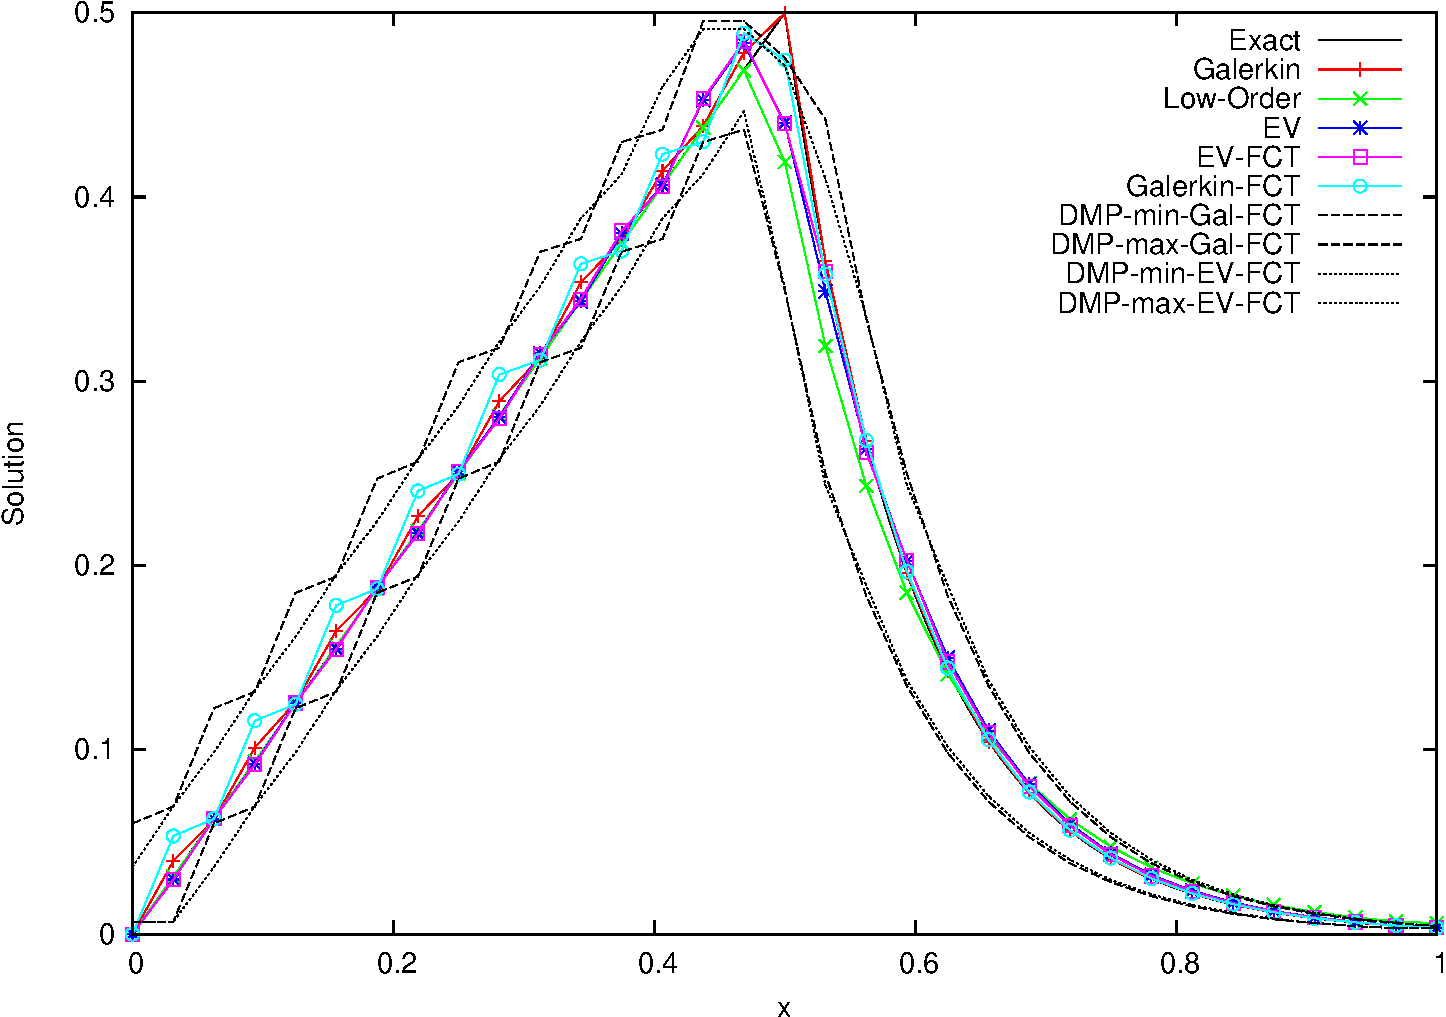
\includegraphics[width=\textwidth]
     {\contentdir/results/transport/source_void_to_absorber/coarse.pdf}
   \caption{Comparison of Solutions for the Source-Void-to-Absorber Problem
     Using SSPRK33 with 32 Cells}
   \label{fig:source_void_to_absorber}
\end{figure}
%-------------------------------------------------------------------------------
\begin{figure}[ht]
   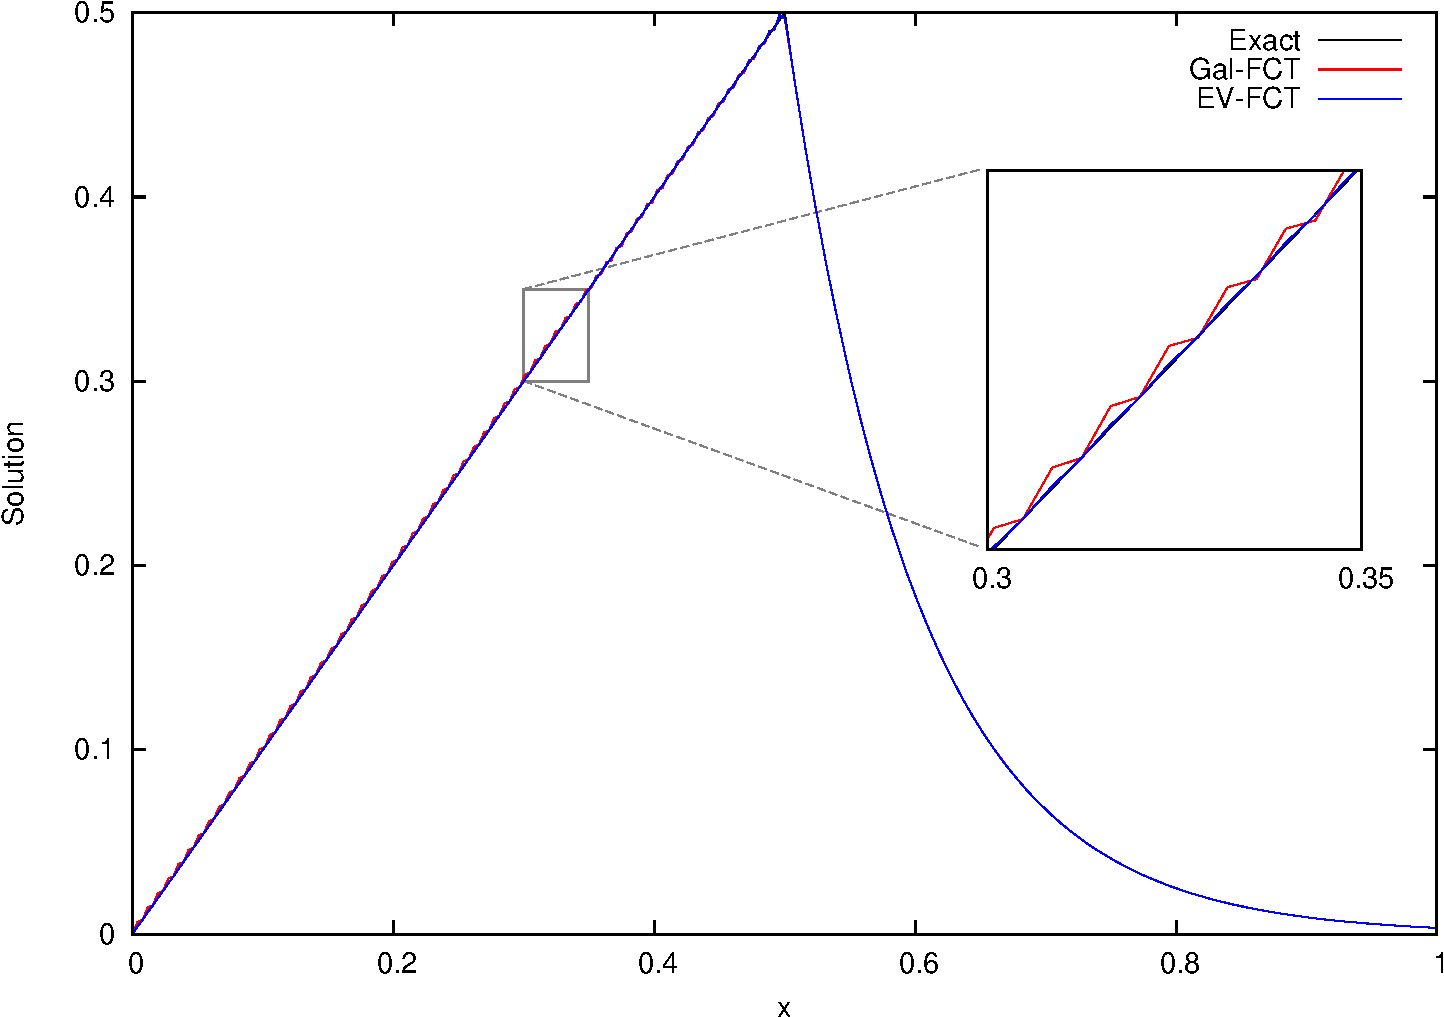
\includegraphics[width=\textwidth]
     {\contentdir/results/transport/source_void_to_absorber/fine.pdf}
   \caption{Comparison of Solutions for the Source-Void-to-Absorber Problem
     Using SSPRK33 with 256 Cells}
   \label{fig:source_void_to_absorber_fine}
\end{figure}
%-------------------------------------------------------------------------------

The steady-state results for this test problem revealed some significant
FCT issues regarding the antidiffusion from Dirichlet nodes.
When Dirichlet boundary conditions are strongly imposed, solution
bounds do not apply, and it becomes unclear how to limit antidiffusion
fluxes from these nodes. Consider symmetric limiters, i.e., those such that
$L\ij=L\ji$, such as Zalesak's limiter, for which
\begin{equation}
  L\ij = \left\{\begin{array}{c c}
    \min(L_i^+,L_j^-) & P\ij > 0\\
    \min(L_i^-,L_j^+) & P\ij < 0\\
  \end{array}\right. \eqp
\end{equation}
Suppose $i$ corresponds to a degree of freedom for which Dirichlet
boundary conditions are strongly imposed. The uncertainty
is the correct way to decide $L_i^+$ and $L_i^-$ since there
are no valid bounds from which to compute these values.
Figures \ref{fig:source_void_to_absorber_strong1} and 
\ref{fig:source_void_to_absorber_strong0} show the solutions obtained
using strongly imposed Dirichlet boundary conditions with these
values set to $L_i^+=L_i^-=1$ and $L_i^+=L_i^-=0$, respectively.
When $L_i^+=L_i^-=1$, the correction flux from the Dirichlet
DoF $i$, which is positive, has only the upper bound for $j$
to consider. The upper bound for $j$, which is inflated above the
analytical solution due to the source, does not restrict this
antidiffusion flux, and thus it is accepted fully to the unphysical
value. Due to the implicitness of the solution bounds, the lower solution
bound for $j$ is computed from this unphysical value and excludes the
possibility of antidiffusion back to the analytical solution. This
process continues with all of the other degrees of freedom.
When instead, $L_i^+=L_i^-=0$, the solution does not lie above
the analytical solution in the source region, but significant peak
clipping appears at the interface between the source and absorber
regions. It should be noted that there are combinations of limiting
coefficient values, each in the range $(0,1)$, that produce a more
accurate solution to this problem (without the peak clipping
and resulting inaccuracy in the absorber region); the problem is that Zalesak's
limiter (and in general, any practical limiter) is not optimal
in the sense that it maximizes the magnitude of antidiffusive flux.
One could in principle solve an optimization problem to select
limiting coefficients that maximize the antidiffusive flux, but this
is very expensive and thus not recommended for general use.

For weakly imposed Dirichlet boundary conditions, solution bounds
still apply, so limiting coefficients may be computed without special
consideration. However, one must now consider the possibility of
inaccurate boundary values.
Figures \ref{fig:source_void_to_absorber_weak} shows the steady-state 
solutions obtained using weakly imposed Dirichlet boundary conditions.
In this case, the antidiffusion flux from the boundary gets limited
(but not fully) due to the lower solution bound of the Dirichlet node.
Because some antidiffusion was accepted here, the peak reaches
a higher value than with the $L_i^+=L_i^-=0$ case.
Finally, Figure \ref{fig:source_void_to_absorber_penalty} shows
the steady-state solution obtained with weakly imposed Dirichlet
boundary conditions and a boundary penalty (see Section \ref{sec:transport_bc}).
The FCT solution looks very similar to the case without any penalty,
but the effect on the low-order and entropy viscosity solutions is
clear.

%-------------------------------------------------------------------------------
\begin{figure}[ht]
   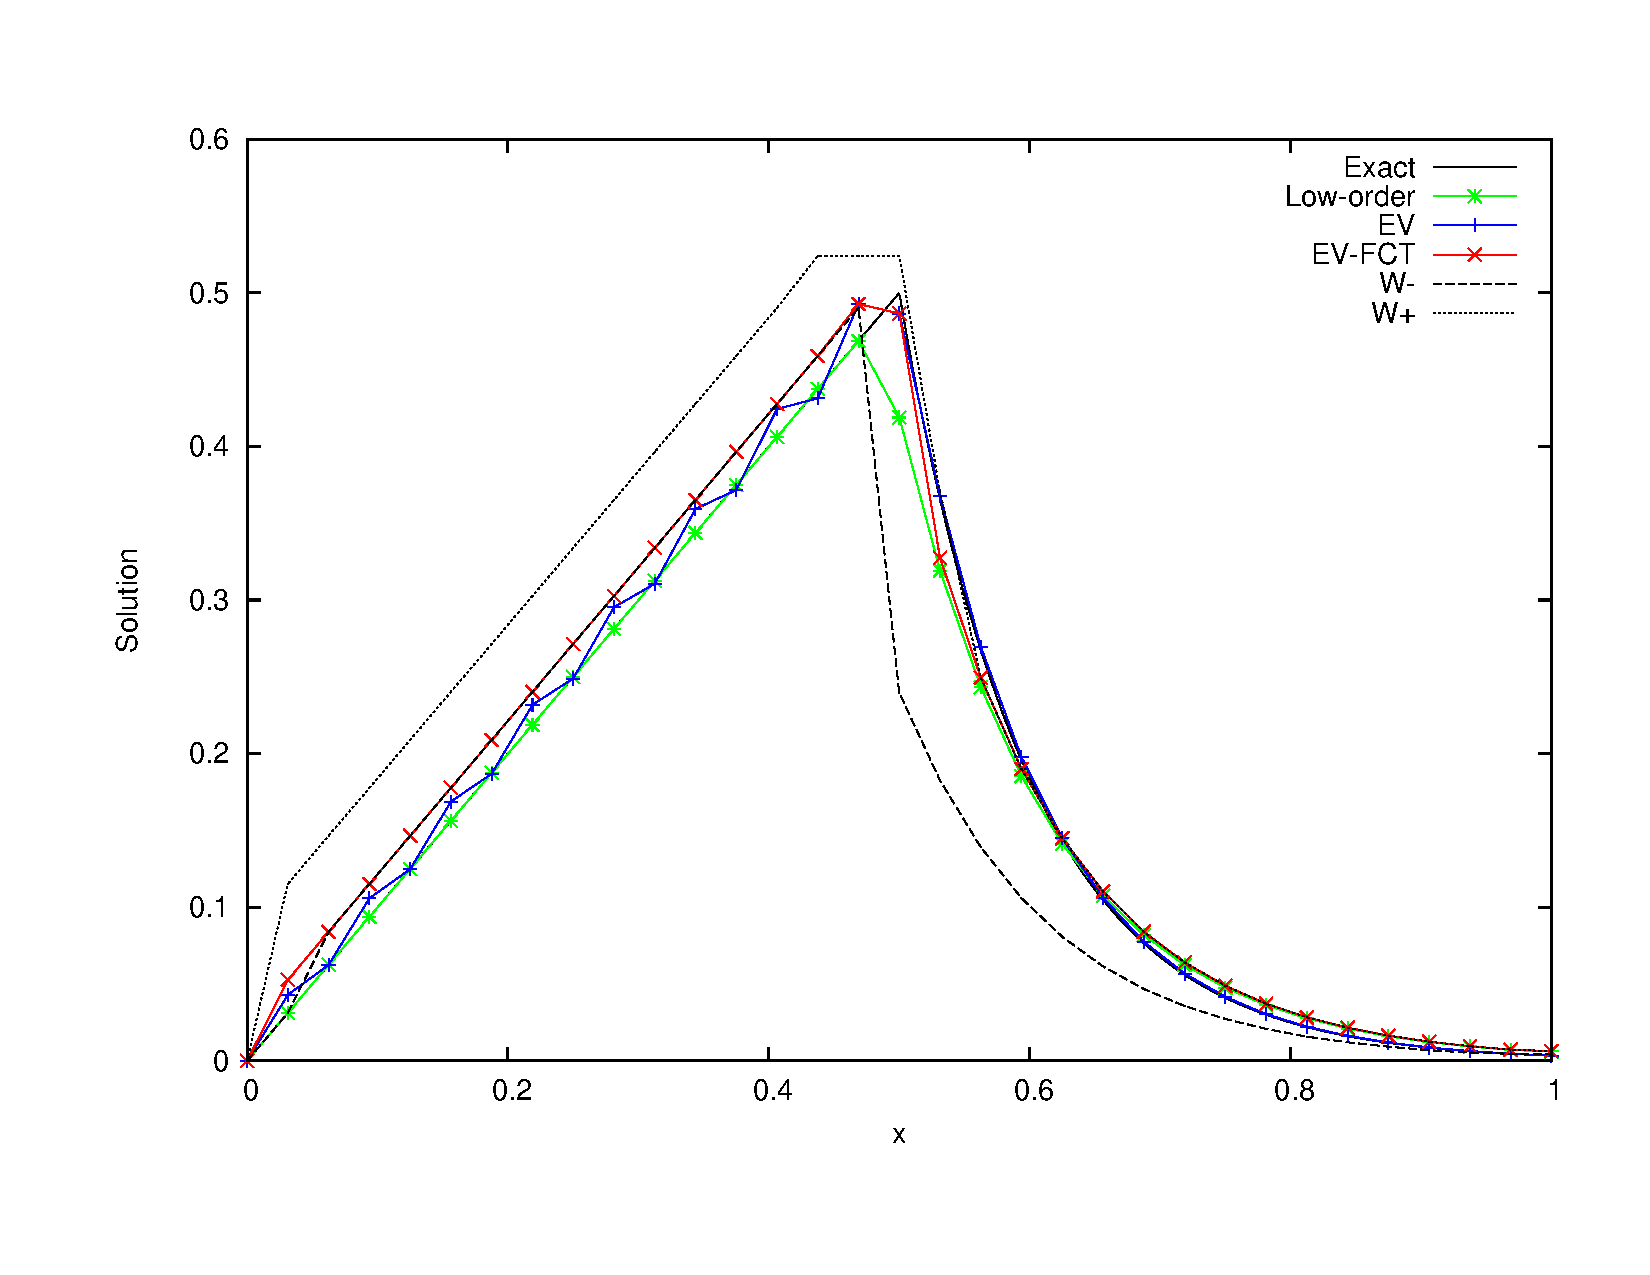
\includegraphics[width=\textwidth]
     {\contentdir/results/transport/source_void_to_absorber/images/strong1.pdf}
   \caption{Steady-State Solutions for the Source-Void-to-Absorber Problem
     with Strongly Imposed Dirichlet Boundary Conditions and $L^-=L^+=1$}
   \label{fig:source_void_to_absorber_strong1}
\end{figure}
%-------------------------------------------------------------------------------
%-------------------------------------------------------------------------------
\begin{figure}[ht]
   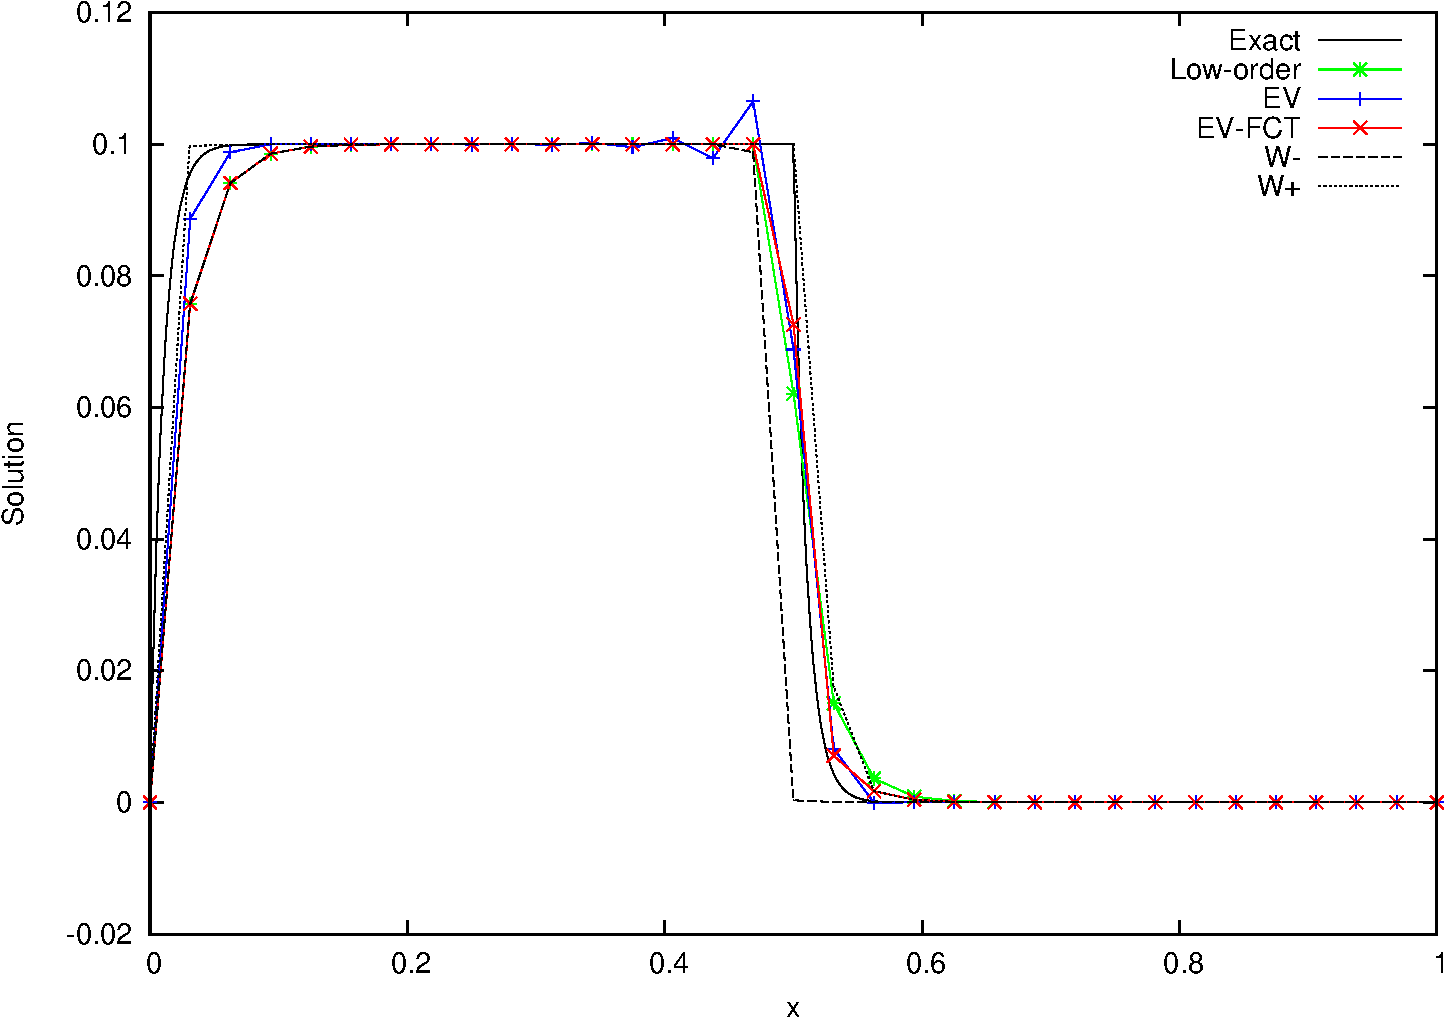
\includegraphics[width=\textwidth]
     {\contentdir/results/transport/source_void_to_absorber/images/strong0.pdf}
   \caption{Steady-State Solutions for the Source-Void-to-Absorber Problem
     with Strongly Imposed Dirichlet Boundary Conditions and $L^-=L^+=0$}
   \label{fig:source_void_to_absorber_strong0}
\end{figure}
%-------------------------------------------------------------------------------
%-------------------------------------------------------------------------------
\begin{figure}[ht]
   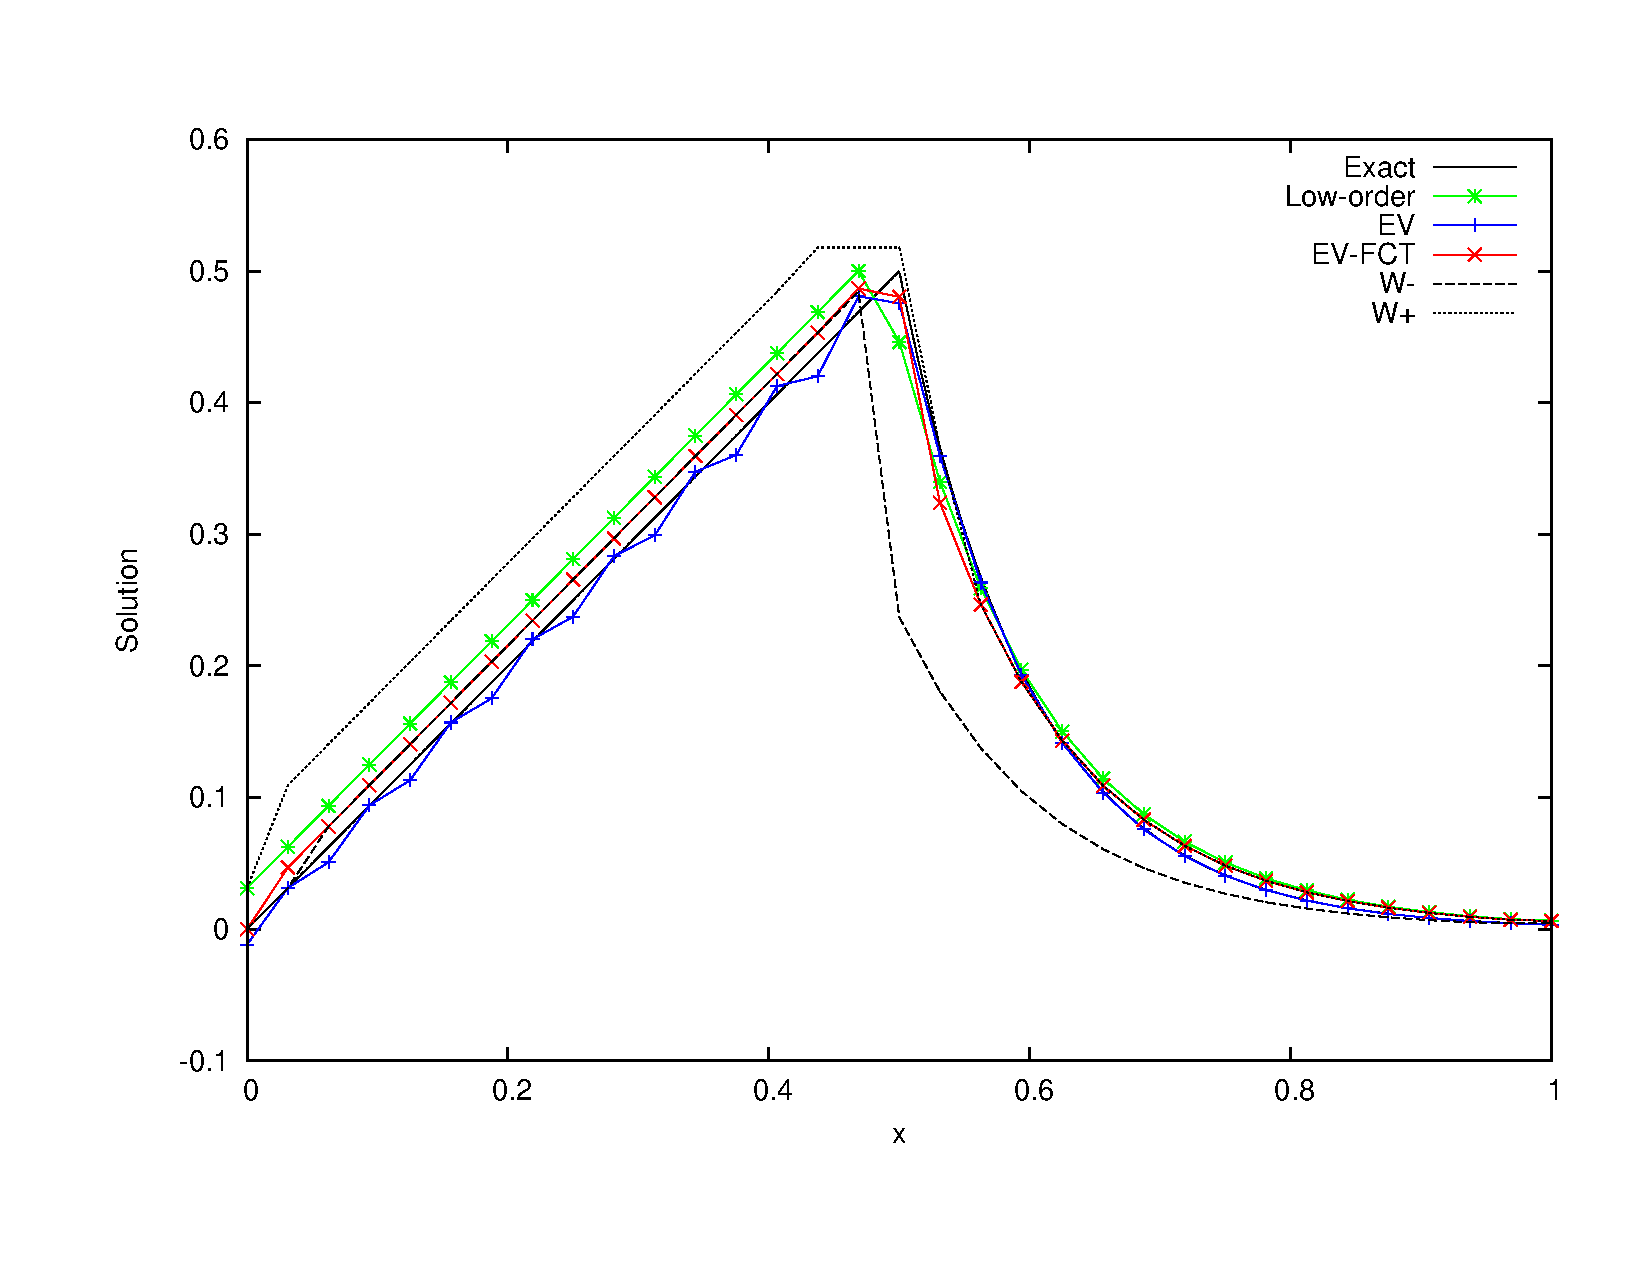
\includegraphics[width=\textwidth]
     {\contentdir/results/transport/source_void_to_absorber/images/weak.pdf}
   \caption{Steady-State Solutions for the Source-Void-to-Absorber Problem
     with Weakly Imposed Dirichlet Boundary Conditions}
   \label{fig:source_void_to_absorber_weak}
\end{figure}
%-------------------------------------------------------------------------------
%-------------------------------------------------------------------------------
\begin{figure}[ht]
   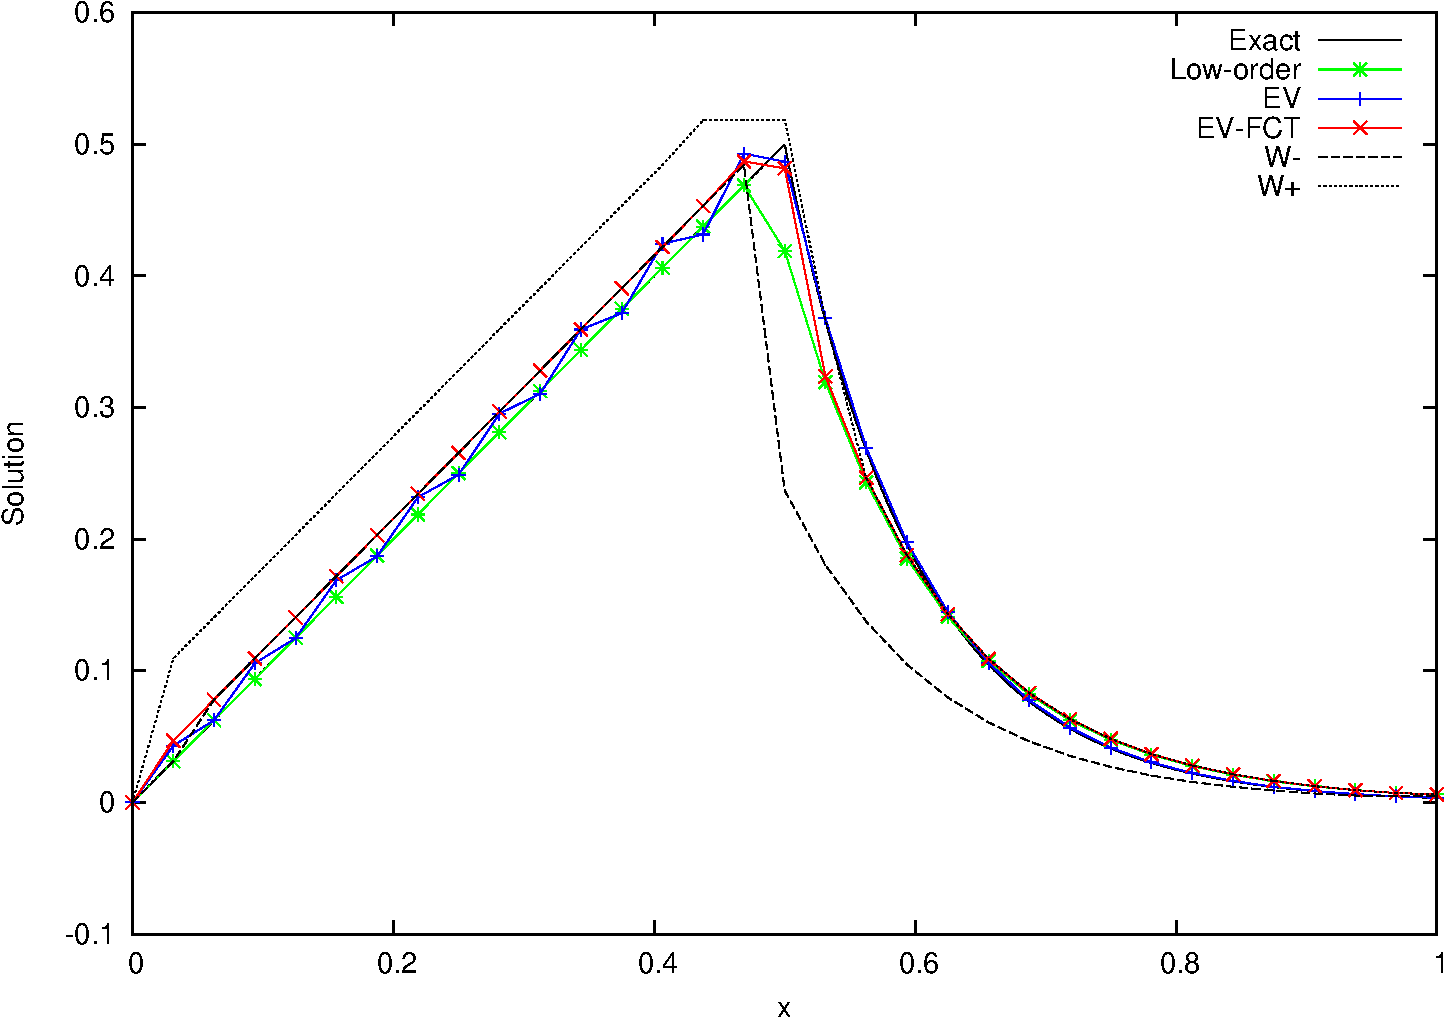
\includegraphics[width=\textwidth]
     {\contentdir/results/transport/source_void_to_absorber/images/weak_with_penalty.pdf}
   \caption{Steady-State Solutions for the Source-Void-to-Absorber Problem
     with Weakly Imposed Dirichlet Boundary Conditions and Boundary Penalty}
   \label{fig:source_void_to_absorber_penalty}
\end{figure}
%-------------------------------------------------------------------------------

Table \ref{tab:source_void_to_absorber_be_iterations_cells} shows the
results of a study of the number of EV and FCT iterations for
BE time discretization, required in
a transient with a constant CFL of 1 and varying mesh sizes. The
results in the table show a decrease in the number of EV iterations
per time step, and a relatively constant number of FCT iterations per
time step.

%-------------------------------------------------------------------------------
\begin{center}
\begin{table}[ht]
\caption{Nonlinear Iterations vs. Number of Cells for the
  Source-Void-to-Absorber Test Problem Using Implicit Euler Time Discretization
  with CFL = 1}
\label{tab:source_void_to_absorber_be_iterations_cells}
\begin{tabular}{c c c c c}\toprule
$N_{cell}$ & \multicolumn{2}{c}{\emph{EV}} & \multicolumn{2}{c}{\emph{FCT}}\\
           & \emph{Total} & \emph{Avg.}    &  \emph{Total} & \emph{Avg.}\\\midrule
  8 &  661 & 24.48 &   244 &  9.04\\
 16 &  807 & 19.21 &   655 & 15.60\\
 32 &  844 & 11.25 &  1194 & 15.92\\
 64 & 1204 &  8.72 &  2024 & 14.67\\
128 & 1752 &  6.59 &  3675 & 13.82\\
256 & 2713 &  5.20 &  6673 & 12.78\\
512 & 4284 &  4.14 & 12098 & 11.69\\
\bottomrule\end{tabular}
\end{table}
\end{center}
%-------------------------------------------------------------------------------

Table \ref{tab:source_void_to_absorber_be_iterations_cfl} shows
the results of a study of nonlinear iterations vs. CFL number for
implicit Euler time discretization and 128 cells. The general
trend shows that entropy viscosity iterations per time step gradually increase
with increasing CFL, while FCT iterations per time step increases
much more quickly. Even more problematic is that the EV-FCT solution
error jumps very quickly from CFLs $\nu=5$ to $\nu=10$.

%-------------------------------------------------------------------------------
\begin{table}[htb]
\caption{Nonlinear Iterations vs. CFL Number for the
 Source-Void-to-Absorber Test Problem Using Implicit Euler Time Discretization
 with 128 Cells}
\label{tab:source_void_to_absorber_be_iterations_cfl}
\centering
\begin{tabular}{c c c c c c c }\toprule
 & & \multicolumn{2}{c}{\emph{EV}}
  & \multicolumn{2}{c}{\emph{FCT}} &\\
\emph{CFL} & $N_{step}$ & \emph{Total} & \emph{Avg.}
  & \emph{Total} & \emph{Avg.} & $L^2$ \emph{err.}\\\midrule
0.1 & 2661 & 15006 &  5.64 & 14036 &   5.27 & $3.013\times10^{-3}$\\
0.5 &  533 &  3445 &  6.46 &  5000 &   9.38 & $3.033\times10^{-3}$\\
1.0 &  266 &  1752 &  6.59 &  3675 &  13.82 & $3.023\times10^{-3}$\\
5.0 &   54 &   471 &  8.72 & 12208 & 226.07 & $2.979\times10^{-3}$\\
10.0 &  27 &   232 &  8.59 &  6126 & 226.89 & $3.325\times10^{-3}$\\
20.0 &  14 &   133 &  9.50 &  3713 & 265.21 & $3.727\times10^{-3}$\\
50.0 &   6 &    62 & 10.33 &  2077 & 346.17 & $7.191\times10^{-3}$\\
\bottomrule\end{tabular}
\end{table}
%-------------------------------------------------------------------------------

\clearpage

In this section, results are presented for the
source-void-to-absorber test problem. This is a 1-D test problem
with zero incoming flux incident on the left boundary,
a constant source in a void in the left half of the
domain, and an absorber with no source in the right half of the
domain. The test problem description is given by Table
\ref{tab:source_void_to_absorber}.

%-------------------------------------------------------------------------------
\begin{table}[htb]\caption{Source-Void-to-Absorber Test Problem Summary}
\label{tab:source_void_to_absorber}
\centering
\begin{tabular}{l l}\toprule
\emph{Parameter} & \emph{Value}\\\midrule
Domain & $\domain = (0,1)$\\
Initial Conditions & $u_0(x)=0$\\
Boundary Conditions & $u(0,t)=0 \eqc \quad t>0$\\
Direction & $\di = \mathbf{e}_x$\\
Cross Section & $\sigma(x)=\left\{\begin{array}{c l}
   0,  & x < \frac{1}{2}\\
   10, & \mbox{otherwise}\end{array}\right.$\\
Source & $q(\x,t)=\left\{\begin{array}{c l}
   1,  & x < \frac{1}{2}\\
   0,  & \mbox{otherwise}\end{array}\right.$\\
Speed & $\speed=1$\\
Exact Solution & $u(x,t)=\left\{\begin{array}{l l}
   \scalarsolution_{\text{ss}}(x), & x-t<0\\
   0, & \mbox{otherwise}
   \end{array}\right.$ \\
   & $\scalarsolution_{\text{ss}}(x) =
       \left\{\begin{array}{l l}
          e^{-10(x-\frac{1}{2})}, & x\ge\frac{1}{2}\\
          1,                      & \mbox{otherwise}
       \end{array}\right.$\\
\bottomrule\end{tabular}
\end{table}
%-------------------------------------------------------------------------------

Figure \ref{fig:source_void_to_absorber}
shows the results for this problem using SSPRK time discretization,
a CFL of 0.5, and 32 cells.
Entropy residual and jump coefficients $\entropyresidualcoef$ and
$\entropyjumpcoef$ are both 1.
Table \ref{tab:source_void_to_absorber_run_parameters} summarizes the
run parameters to generate the results in this section.
Figure \ref{fig:source_void_to_absorber_fine} shows results
for a finer mesh (256 cells) that illustrates the shortcomings of Galerkin-FCT
vs. EV-FCT: Galerkin-FCT does not necessarily converge to the
entropy solution.

%-------------------------------------------------------------------------------
\begin{table}[ht]\caption{Source-Void-to-Absorber Test Problem Run Parameters}
\label{tab:source_void_to_absorber_run_parameters}
\centering
\begin{tabular}{l l}\toprule
\emph{Parameter} & \emph{Value}\\\midrule
Number of Cells & $N_{cell} = 32, 256$\\
End Time & $t = 1$\\
CFL Number & $\nu = 0.5$\\\midrule
Entropy Function & $\entropy(u) = \frac{1}{2}u^2$\\
Entropy Residual Coefficient & $\entropyresidualcoef = 1$\\
Entropy Jump Coefficient & $\entropyjumpcoef = 1$\\
\bottomrule\end{tabular}
\end{table}
%-------------------------------------------------------------------------------
\begin{figure}[ht]
   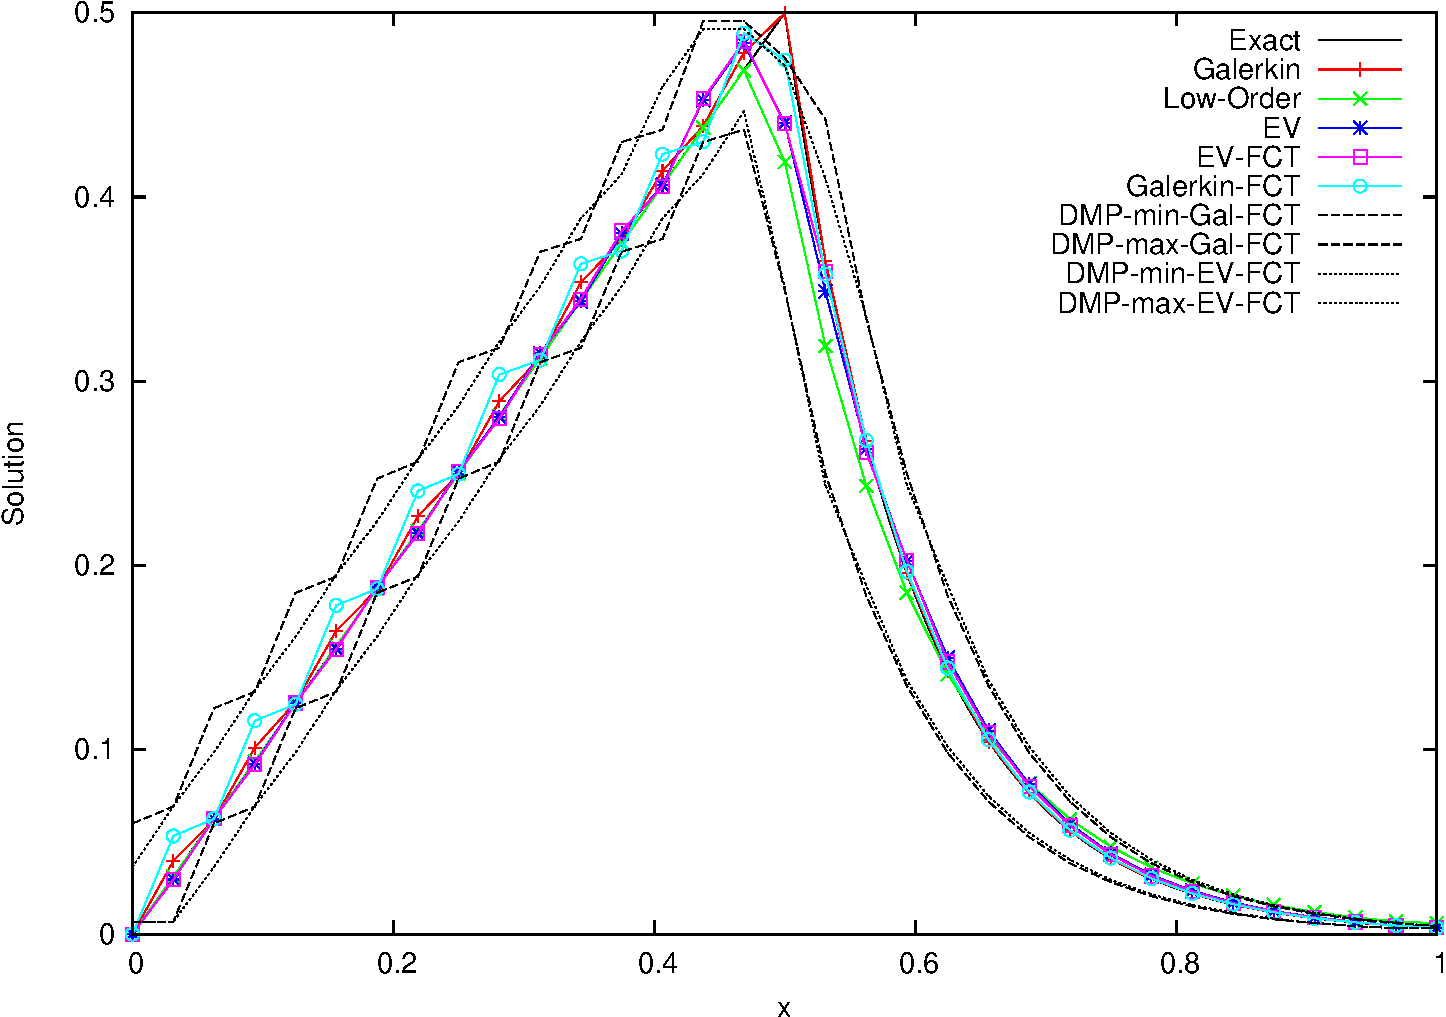
\includegraphics[width=\textwidth]
     {\contentdir/results/transport/source_void_to_absorber/coarse.pdf}
   \caption{Comparison of Solutions for the Source-Void-to-Absorber Problem
     Using SSPRK33 with 32 Cells}
   \label{fig:source_void_to_absorber}
\end{figure}
%-------------------------------------------------------------------------------
\begin{figure}[ht]
   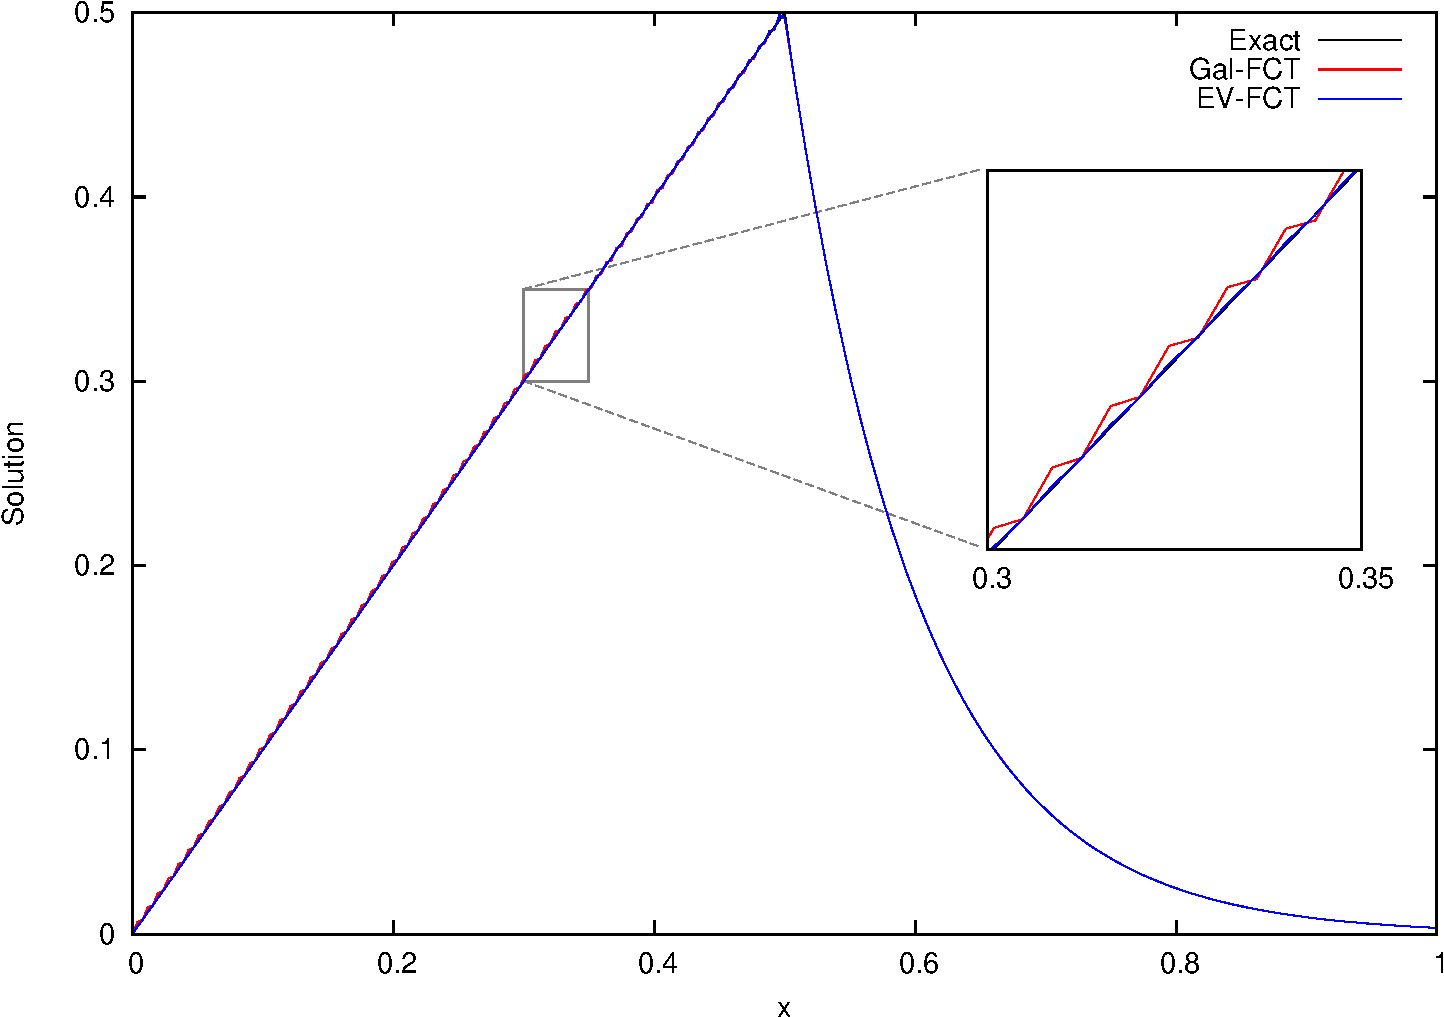
\includegraphics[width=\textwidth]
     {\contentdir/results/transport/source_void_to_absorber/fine.pdf}
   \caption{Comparison of Solutions for the Source-Void-to-Absorber Problem
     Using SSPRK33 with 256 Cells}
   \label{fig:source_void_to_absorber_fine}
\end{figure}
%-------------------------------------------------------------------------------

The steady-state results for this test problem revealed some significant
FCT issues regarding the antidiffusion from Dirichlet nodes.
When Dirichlet boundary conditions are strongly imposed, solution
bounds do not apply, and it becomes unclear how to limit antidiffusion
fluxes from these nodes. Consider symmetric limiters, i.e., those such that
$L\ij=L\ji$, such as Zalesak's limiter, for which
\begin{equation}
  L\ij = \left\{\begin{array}{c c}
    \min(L_i^+,L_j^-) & P\ij > 0\\
    \min(L_i^-,L_j^+) & P\ij < 0\\
  \end{array}\right. \eqp
\end{equation}
Suppose $i$ corresponds to a degree of freedom for which Dirichlet
boundary conditions are strongly imposed. The uncertainty
is the correct way to decide $L_i^+$ and $L_i^-$ since there
are no valid bounds from which to compute these values.
Figures \ref{fig:source_void_to_absorber_strong1} and 
\ref{fig:source_void_to_absorber_strong0} show the solutions obtained
using strongly imposed Dirichlet boundary conditions with these
values set to $L_i^+=L_i^-=1$ and $L_i^+=L_i^-=0$, respectively.
When $L_i^+=L_i^-=1$, the correction flux from the Dirichlet
DoF $i$, which is positive, has only the upper bound for $j$
to consider. The upper bound for $j$, which is inflated above the
analytical solution due to the source, does not restrict this
antidiffusion flux, and thus it is accepted fully to the unphysical
value. Due to the implicitness of the solution bounds, the lower solution
bound for $j$ is computed from this unphysical value and excludes the
possibility of antidiffusion back to the analytical solution. This
process continues with all of the other degrees of freedom.
When instead, $L_i^+=L_i^-=0$, the solution does not lie above
the analytical solution in the source region, but significant peak
clipping appears at the interface between the source and absorber
regions. It should be noted that there are combinations of limiting
coefficient values, each in the range $(0,1)$, that produce a more
accurate solution to this problem (without the peak clipping
and resulting inaccuracy in the absorber region); the problem is that Zalesak's
limiter (and in general, any practical limiter) is not optimal
in the sense that it maximizes the magnitude of antidiffusive flux.
One could in principle solve an optimization problem to select
limiting coefficients that maximize the antidiffusive flux, but this
is very expensive and thus not recommended for general use.

For weakly imposed Dirichlet boundary conditions, solution bounds
still apply, so limiting coefficients may be computed without special
consideration. However, one must now consider the possibility of
inaccurate boundary values.
Figures \ref{fig:source_void_to_absorber_weak} shows the steady-state 
solutions obtained using weakly imposed Dirichlet boundary conditions.
In this case, the antidiffusion flux from the boundary gets limited
(but not fully) due to the lower solution bound of the Dirichlet node.
Because some antidiffusion was accepted here, the peak reaches
a higher value than with the $L_i^+=L_i^-=0$ case.
Finally, Figure \ref{fig:source_void_to_absorber_penalty} shows
the steady-state solution obtained with weakly imposed Dirichlet
boundary conditions and a boundary penalty (see Section \ref{sec:transport_bc}).
The FCT solution looks very similar to the case without any penalty,
but the effect on the low-order and entropy viscosity solutions is
clear.

%-------------------------------------------------------------------------------
\begin{figure}[ht]
   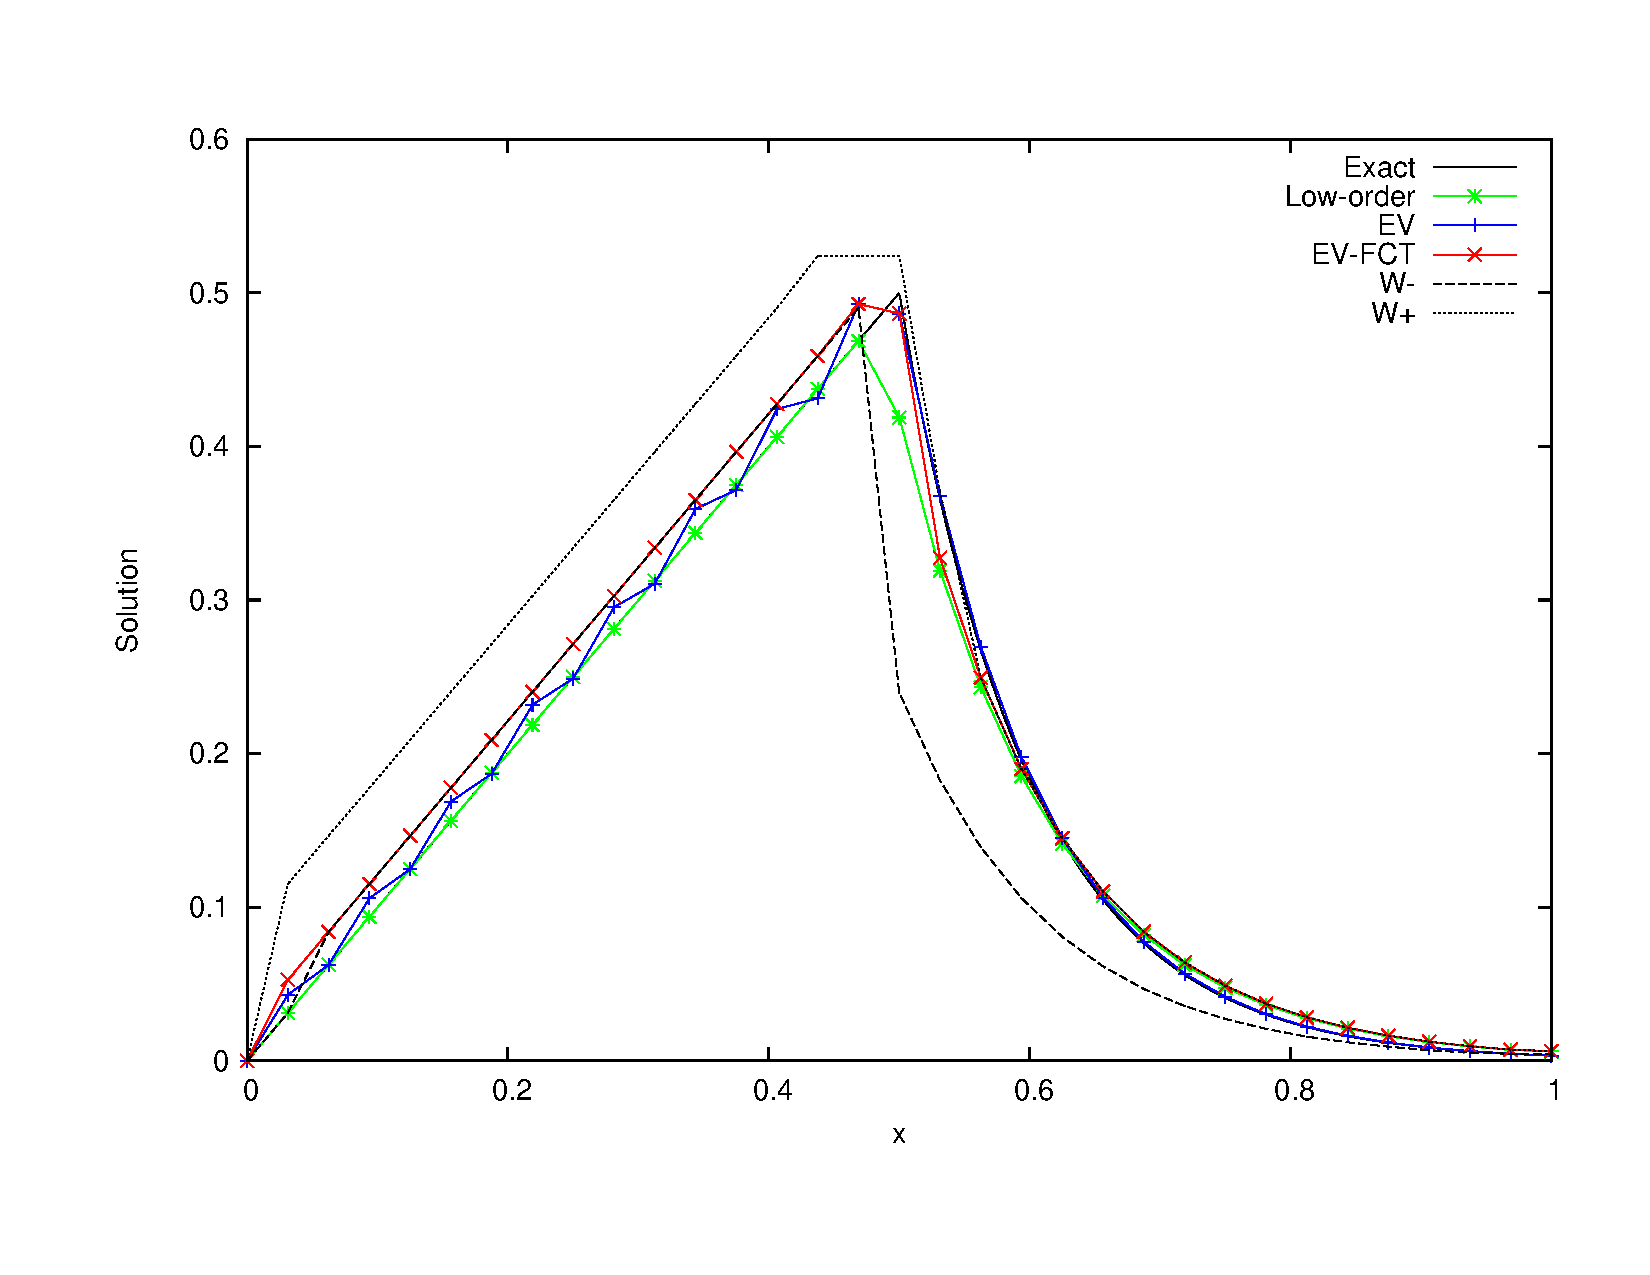
\includegraphics[width=\textwidth]
     {\contentdir/results/transport/source_void_to_absorber/images/strong1.pdf}
   \caption{Steady-State Solutions for the Source-Void-to-Absorber Problem
     with Strongly Imposed Dirichlet Boundary Conditions and $L^-=L^+=1$}
   \label{fig:source_void_to_absorber_strong1}
\end{figure}
%-------------------------------------------------------------------------------
%-------------------------------------------------------------------------------
\begin{figure}[ht]
   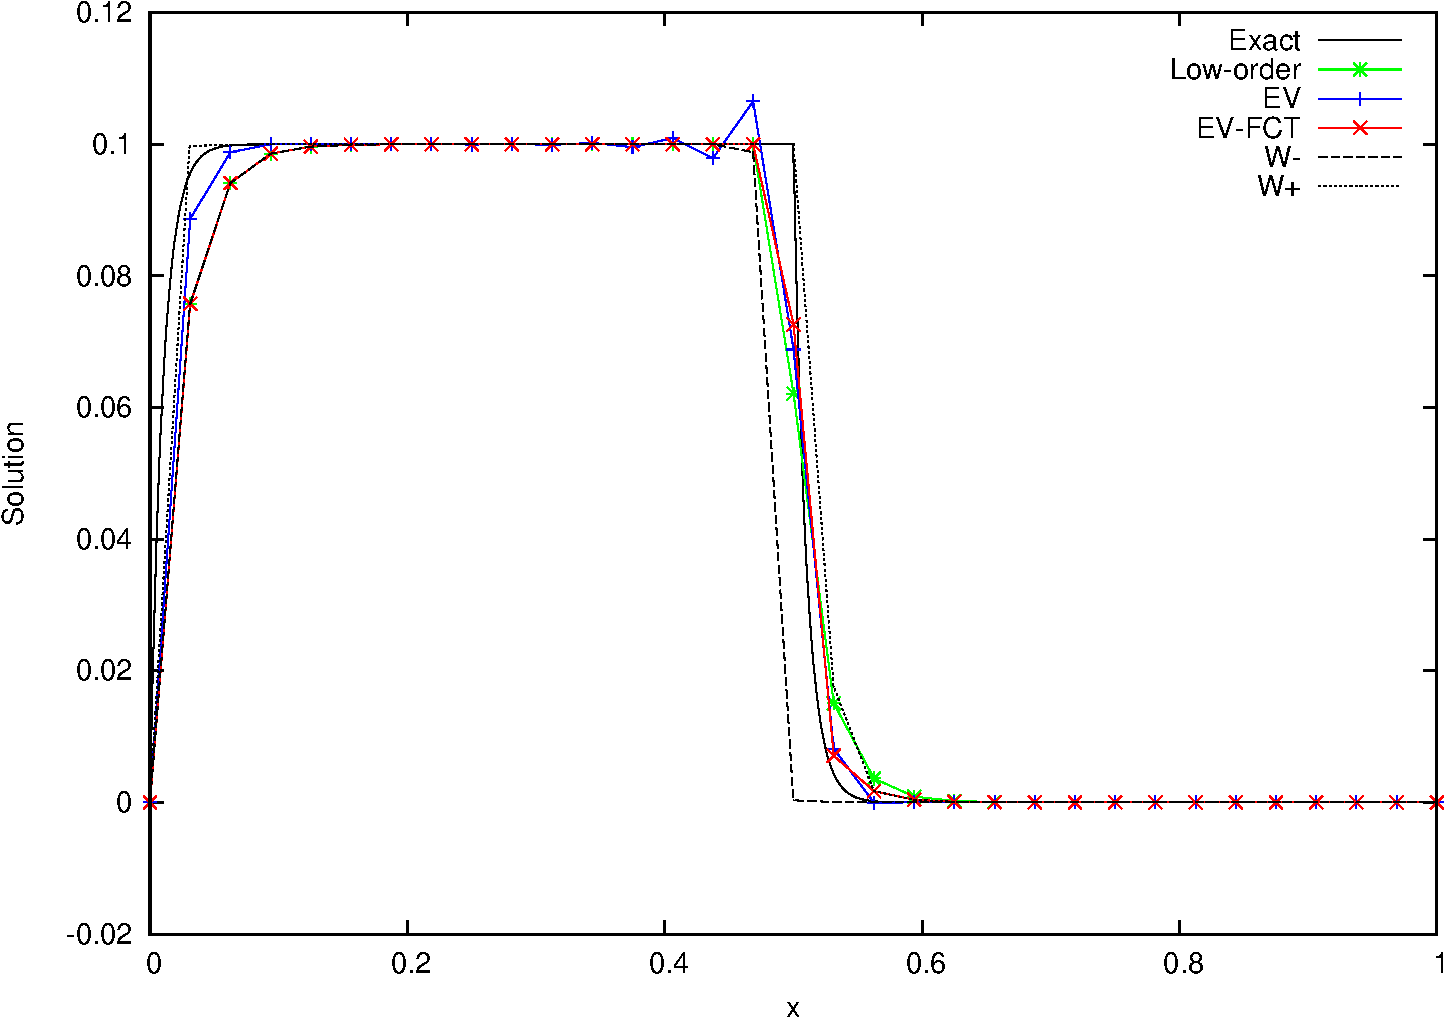
\includegraphics[width=\textwidth]
     {\contentdir/results/transport/source_void_to_absorber/images/strong0.pdf}
   \caption{Steady-State Solutions for the Source-Void-to-Absorber Problem
     with Strongly Imposed Dirichlet Boundary Conditions and $L^-=L^+=0$}
   \label{fig:source_void_to_absorber_strong0}
\end{figure}
%-------------------------------------------------------------------------------
%-------------------------------------------------------------------------------
\begin{figure}[ht]
   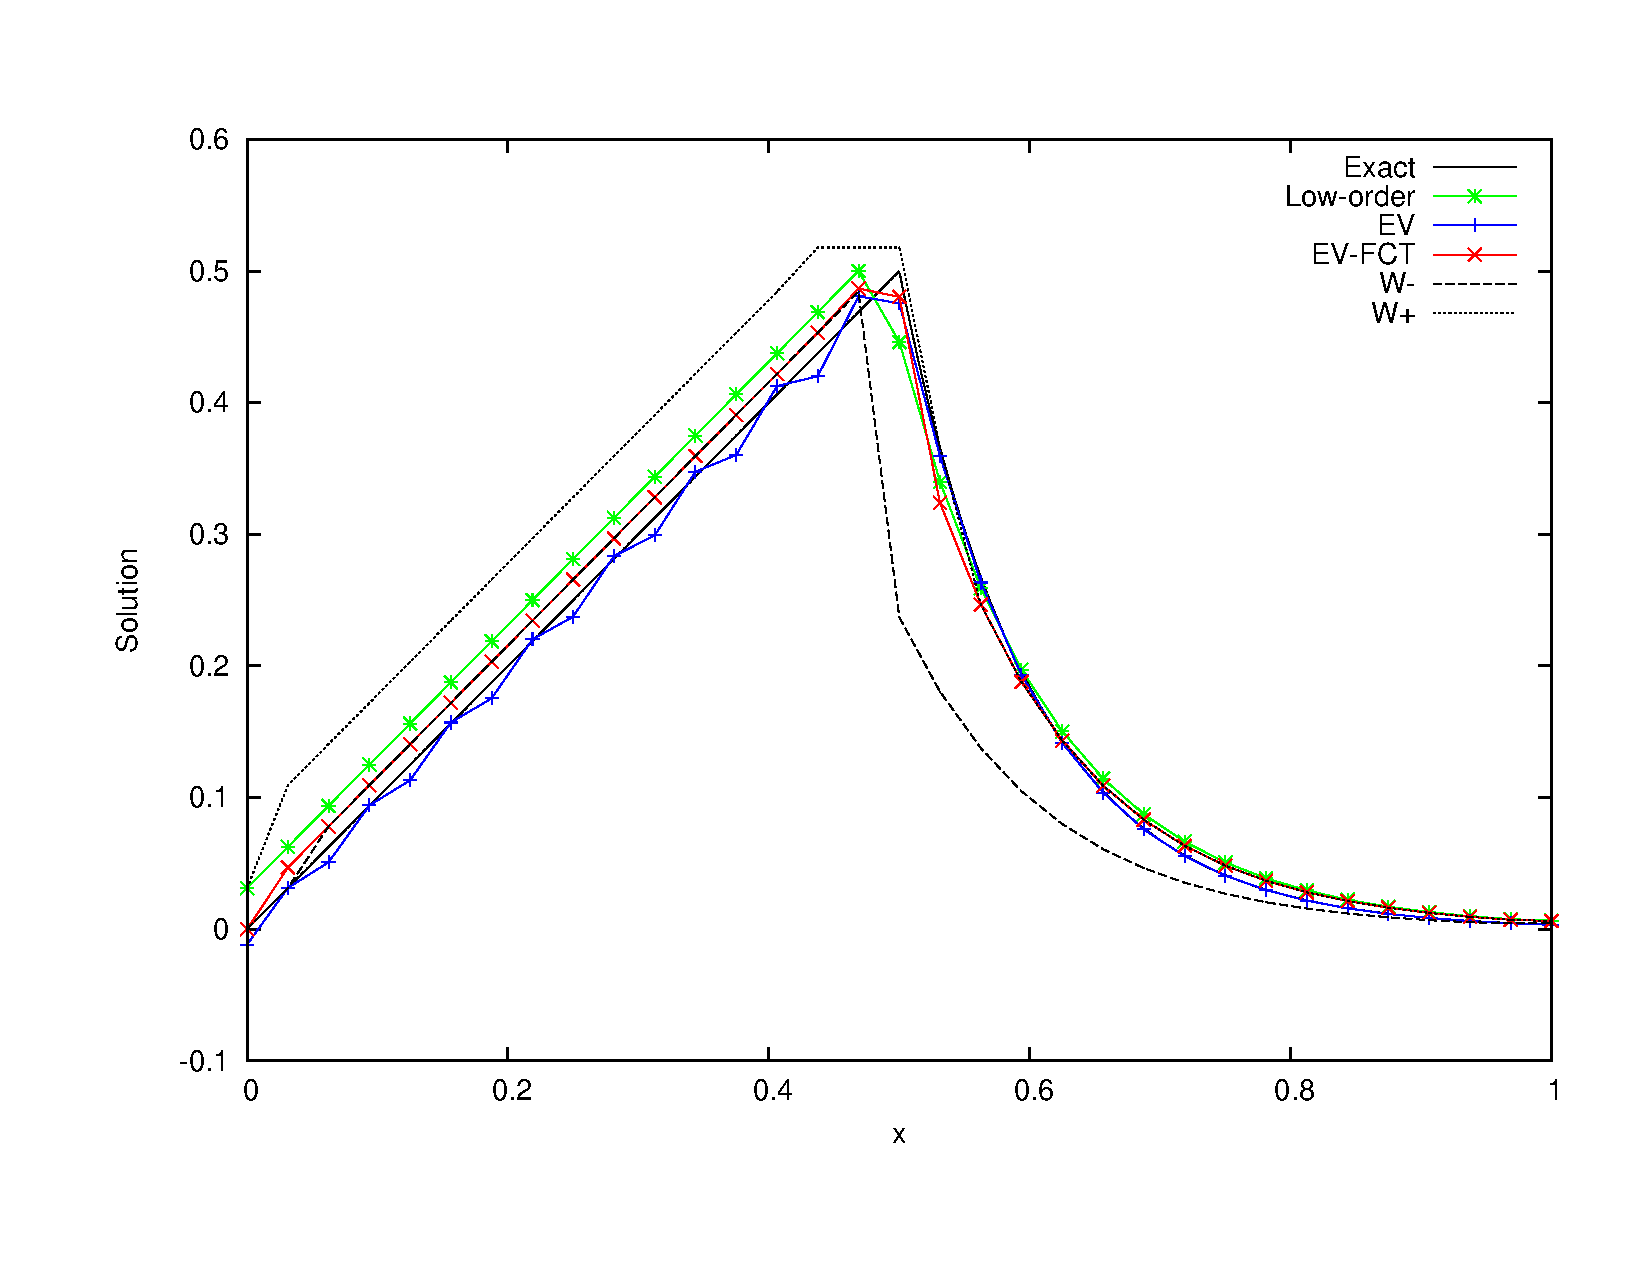
\includegraphics[width=\textwidth]
     {\contentdir/results/transport/source_void_to_absorber/images/weak.pdf}
   \caption{Steady-State Solutions for the Source-Void-to-Absorber Problem
     with Weakly Imposed Dirichlet Boundary Conditions}
   \label{fig:source_void_to_absorber_weak}
\end{figure}
%-------------------------------------------------------------------------------
%-------------------------------------------------------------------------------
\begin{figure}[ht]
   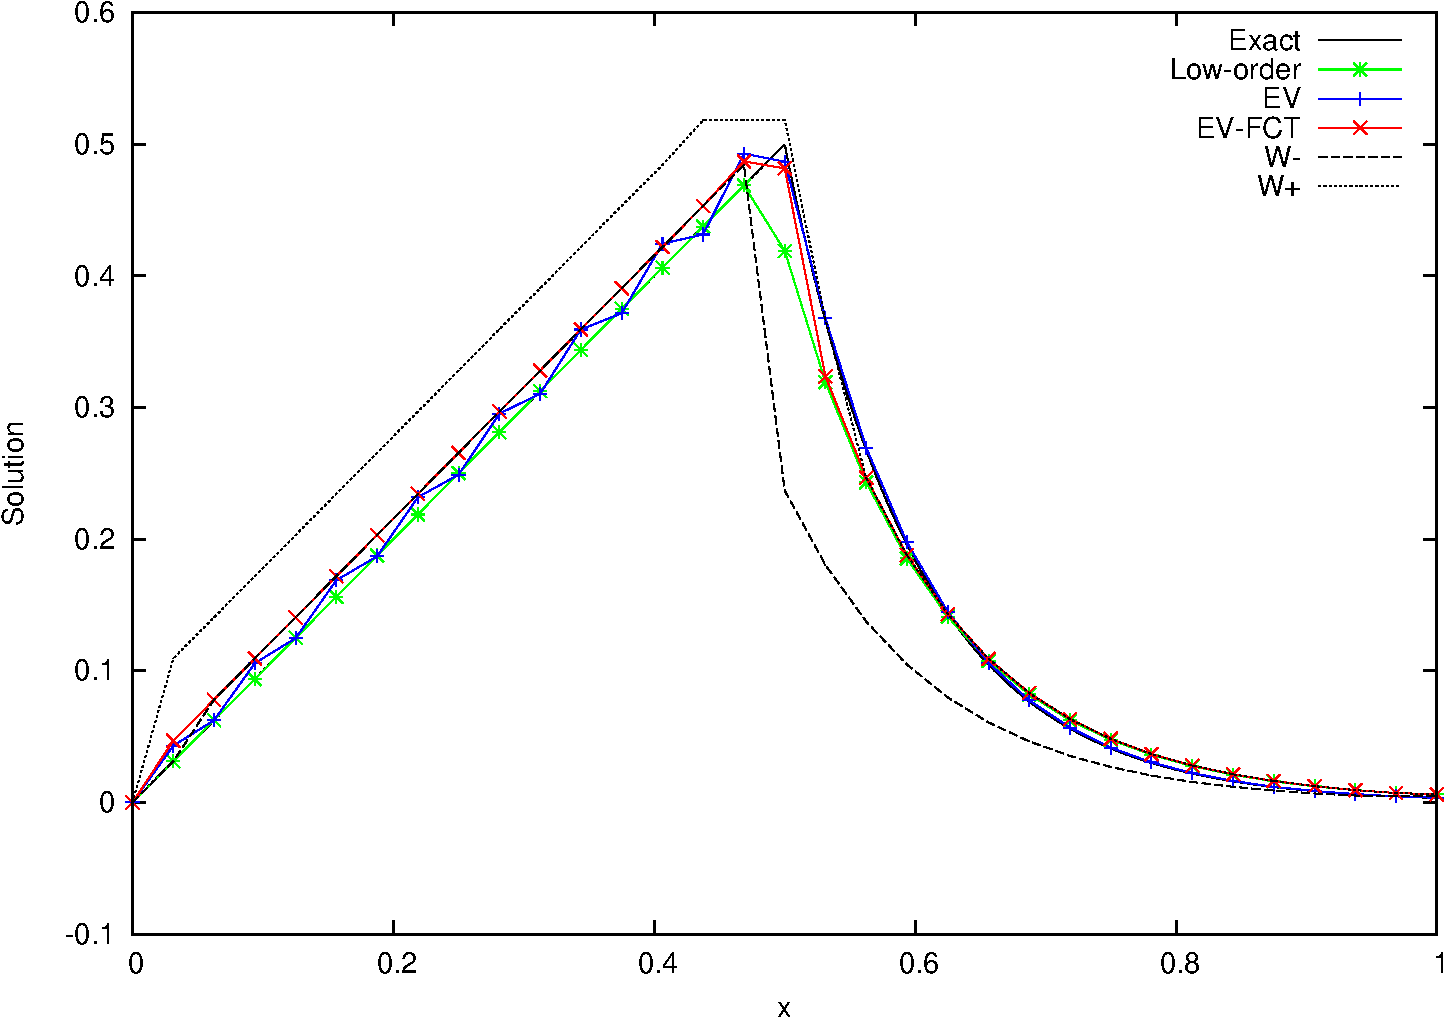
\includegraphics[width=\textwidth]
     {\contentdir/results/transport/source_void_to_absorber/images/weak_with_penalty.pdf}
   \caption{Steady-State Solutions for the Source-Void-to-Absorber Problem
     with Weakly Imposed Dirichlet Boundary Conditions and Boundary Penalty}
   \label{fig:source_void_to_absorber_penalty}
\end{figure}
%-------------------------------------------------------------------------------

Table \ref{tab:source_void_to_absorber_be_iterations_cells} shows the
results of a study of the number of EV and FCT iterations for
BE time discretization, required in
a transient with a constant CFL of 1 and varying mesh sizes. The
results in the table show a decrease in the number of EV iterations
per time step, and a relatively constant number of FCT iterations per
time step.

%-------------------------------------------------------------------------------
\begin{center}
\begin{table}[ht]
\caption{Nonlinear Iterations vs. Number of Cells for the
  Source-Void-to-Absorber Test Problem Using Implicit Euler Time Discretization
  with CFL = 1}
\label{tab:source_void_to_absorber_be_iterations_cells}
\begin{tabular}{c c c c c}\toprule
$N_{cell}$ & \multicolumn{2}{c}{\emph{EV}} & \multicolumn{2}{c}{\emph{FCT}}\\
           & \emph{Total} & \emph{Avg.}    &  \emph{Total} & \emph{Avg.}\\\midrule
  8 &  661 & 24.48 &   244 &  9.04\\
 16 &  807 & 19.21 &   655 & 15.60\\
 32 &  844 & 11.25 &  1194 & 15.92\\
 64 & 1204 &  8.72 &  2024 & 14.67\\
128 & 1752 &  6.59 &  3675 & 13.82\\
256 & 2713 &  5.20 &  6673 & 12.78\\
512 & 4284 &  4.14 & 12098 & 11.69\\
\bottomrule\end{tabular}
\end{table}
\end{center}
%-------------------------------------------------------------------------------

Table \ref{tab:source_void_to_absorber_be_iterations_cfl} shows
the results of a study of nonlinear iterations vs. CFL number for
implicit Euler time discretization and 128 cells. The general
trend shows that entropy viscosity iterations per time step gradually increase
with increasing CFL, while FCT iterations per time step increases
much more quickly. Even more problematic is that the EV-FCT solution
error jumps very quickly from CFLs $\nu=5$ to $\nu=10$.

%-------------------------------------------------------------------------------
\begin{table}[htb]
\caption{Nonlinear Iterations vs. CFL Number for the
 Source-Void-to-Absorber Test Problem Using Implicit Euler Time Discretization
 with 128 Cells}
\label{tab:source_void_to_absorber_be_iterations_cfl}
\centering
\begin{tabular}{c c c c c c c }\toprule
 & & \multicolumn{2}{c}{\emph{EV}}
  & \multicolumn{2}{c}{\emph{FCT}} &\\
\emph{CFL} & $N_{step}$ & \emph{Total} & \emph{Avg.}
  & \emph{Total} & \emph{Avg.} & $L^2$ \emph{err.}\\\midrule
0.1 & 2661 & 15006 &  5.64 & 14036 &   5.27 & $3.013\times10^{-3}$\\
0.5 &  533 &  3445 &  6.46 &  5000 &   9.38 & $3.033\times10^{-3}$\\
1.0 &  266 &  1752 &  6.59 &  3675 &  13.82 & $3.023\times10^{-3}$\\
5.0 &   54 &   471 &  8.72 & 12208 & 226.07 & $2.979\times10^{-3}$\\
10.0 &  27 &   232 &  8.59 &  6126 & 226.89 & $3.325\times10^{-3}$\\
20.0 &  14 &   133 &  9.50 &  3713 & 265.21 & $3.727\times10^{-3}$\\
50.0 &   6 &    62 & 10.33 &  2077 & 346.17 & $7.191\times10^{-3}$\\
\bottomrule\end{tabular}
\end{table}
%-------------------------------------------------------------------------------

\clearpage

\end{document}


%###############################################################################
\section{Research Goals\label{sec:goals}}
%###############################################################################
The main goal of this research is to develop numerical methods for hyperbolic
PDEs that address the development of spurious oscillations and negativities for
physically positive solution quantities. The equations and models under
consideration are the scalar transport PDE model given in Section
\ref{sec:scalar_model} and the shallow water equations (SWE) with flat bottom
topography ($\nabla\bathymetry=\mathbf{0}$), given in Section
\ref{sec:sw_model}.  The methodology developed for these equations is intended
to be largely extendible to other hyperbolic systems. The following list
discusses specific research objectives that derive from the main research goal.

\begin{itemize}
  \item \textbf{Develop low-order scheme.}
    For the scalar case, this first-order-accurate scheme should satisfy a discrete maximum principle
    as described in Section \ref{sec:low_order_scheme}. For the systems case,
    this scheme should have an invariant domain. The domain-invariant scheme
    is developed for general conservation law systems; however, the scheme
    requires an estimation of maximum wave speeds, which entails an
    analysis of the characteristics for the specific hyperbolic system. This
    research performs this analysis for the shallow water equations with flat
    bottom topography. The monotonicity and
    positivity-preservation of these schemes should be demonstrated with
    numerical examples.

    For the \emph{scalar} case, the low-order scheme should be
    developed for the following time discretizations:
    \begin{itemize}
      \item steady-state,
      \item implicit $\theta$ methods: implicit Euler and Crank-Nicolson,
      \item explicit methods of the SSPRK family.
    \end{itemize}
    For the \emph{systems} case, the low-order scheme should be
    developed for the following time discretizations:
    \begin{itemize}
      \item explicit methods of the SSPRK family.
    \end{itemize}
  \item \textbf{Develop high-order entropy-based scheme.}
    The entropy-based scheme should be second-order-accurate and should
    demonstrate stability with numerical examples. A reduction in the occurrence
    and magnitude of spurious oscillations should be observed. The scalar
    case will use an arbitrary convex entropy function such as
    $\entropy(\scalarsolution)=\half\scalarsolution^2$, while for the shallow
    water equations, the entropy function will be the total energy.

    For the \emph{scalar} case, the high-order scheme should be
    developed for the following time discretizations:
    \begin{itemize}
      \item steady-state,
      \item implicit $\theta$ methods: implicit Euler and Crank-Nicolson,
      \item explicit methods of the SSPRK family.
    \end{itemize}
    For the \emph{systems} case, the high-order scheme should be
    developed for the following time discretizations:
    \begin{itemize}
      \item explicit methods of the SSPRK family.
    \end{itemize}
  \item \textbf{Develop Galerkin FCT scheme.}
    The basic FEM-FCT scheme, as described by Kuzmin in \cite{kuzmin_FCT}, should
    be implemented. This scheme uses the standard second-order-accurate Galerkin
    scheme as the high-order scheme in the algorithm. Positivity-preservation and
    a reduction of spurious oscillations should be demonstrated.

    For the \emph{scalar} case, the Galerkin FCT scheme should be
    developed for the following time discretizations:
    \begin{itemize}
      \item steady-state,
      \item implicit $\theta$ methods: implicit Euler and Crank-Nicolson,
      \item explicit methods of the SSPRK family.
    \end{itemize}
    For the \emph{systems} case, the Galerkin FCT scheme should be
    developed for the following time discretizations:
    \begin{itemize}
      \item explicit methods of the SSPRK family.
    \end{itemize}
  \item \textbf{Develop entropy-based FCT scheme.}
    The basic FEM-FCT scheme should be modified to replace the Galerkin scheme
    with the high-order entropy-based scheme in the FCT algorithm. This should
    demonstrate positivity-preservation and a further reduction in spurious
    oscillations from the entropy-based method alone.

    For the \emph{scalar} case, the entropy-based FCT scheme should be
    developed for the following time discretizations:
    \begin{itemize}
      \item steady-state,
      \item implicit $\theta$ methods: implicit Euler and Crank-Nicolson,
      \item explicit methods of the SSPRK family.
    \end{itemize}
    For the \emph{systems} case, the entropy-based FCT scheme should be
    developed for the following time discretizations:
    \begin{itemize}
      \item explicit methods of the SSPRK family.
    \end{itemize}
  \item \textbf{Compare schemes.}
    Schemes developed in this research should be compared in a number of
    test problems. In addition to comparing accuracy and convergence rates,
    it is advantageous to determine rough computational cost estimates
    of each method, since the developed methods have the cost of additional
    complexity.
\end{itemize}



%###############################################################################
\section{Conclusions\label{sec:conclusions}}
%###############################################################################
The FCT scheme described in this paper is second-order accurate in space,
converges to the entropy solution, and preserves non-negativity.
Spurious oscillations are mitigated but are not guaranteed to be
eliminated, as smaller magnitude oscillations may exist within the imposed
solution bounds.

% Local solution bounds imposed in the FCT algorithm were derived using the method
% of characteristics and integral transport equation.
% Two sets of solution
% bounds were considered, one considering only values along the upstream
% line segment traversed in a time step, and the other considering a spherical
% neighborhood that encompasses this line segment. The former set of solution
% bounds is much tighter, which has the advantage that there is a smaller range
% of limiting coefficient values that can be used, but has the disadvantage that
% there is less room for antidiffusion.

The traditional FCT phenomenon known as ``stair-stepping'',
``terracing'', or ``plateauing'' is still an open issue, particularly for
fully explicit temporal discretizations; however, these effects
have been shown to diminish or disappear when using SSPRK33 as opposed
to explicit Euler. In addition, these effects are less pronounced for EV-FCT
than in the classic FEM-FCT scheme, which uses the standard Galerkin method as
the high-order method in FCT.

The explicit temporal discretizations of the described FCT scheme yield a
relatively robust algorithm; however, implicit and steady-state discretizations
are much less robust, suffering from severe nonlinear convergence difficulties
in some problems. Implicit schemes become increasingly divergent as the CFL
number is increased. The main complication with implicit and steady-state
FCT schemes is that the imposed solution bounds are implicit with the solution,
and thus the imposed solution bounds change with each iteration of the
nonlinear solver.


%###############################################################################
\bibliographystyle{plain}
\bibliography{\refdir/references}
%###############################################################################

\end{document}
